
\documentclass[../main]{subfiles}
\ifSubfilesClassLoaded{
    \dominitoc
    \tableofcontentsfile
}{}
\begin{document}
%\graphicspath{{\subfix{/02-Architectures/figures}}}
\graphicspath{{./figures},{02-Architectures/figures}}
\chapter{Architectures de cartes auto-organisatrices}
\minitoc

Nous nous concentrerons dans cette thèse sur la création d'architectures de cartes auto-organisatrices ou SOM (\emph{Self-Organizing Maps}) comme modules d'une architecture décentralisée.
Les cartes auto-organisatrices et notamment le modèle de Kohonen sont largement utilisées en tant qu'algorithme d'apprentissage non supervisé appliqué à des tâches de réduction de dimension, de visualisation de données ou de classification.
Cependant, peu de travaux ont exploré l'idée de les assembler en architecture comportant des rétroactions, formant ainsi un système dynamique. 
L'aspect bio-inspiré des cartes de Kohonen et la présence de motifs auto-organisés motivent pourtant cet axe d'utilisation en tant que système dynamique.
% Kohonen écrivait par exemple dans son livre à propos des enjeux des cartes de Kohonen en 1995:
% \begin{quote}
% Un objectif à long terme de l'auto-organisation est de créer des systèmes autonomes dont les éléments se contrôlent mutuellement et apprennent les uns des autres. De tels éléments de contrôle peuvent être implémentés par des SOMs spécifiques; le problème principal est alors l'interface, en particulier la mise à l'échelle automatique des signaux d'interconnexion entre les modules et la collecte de signaux pertinents comme interface entre les modules. Nous laisserons cette idée aux recherches futures.
% \cite{Kohonen1995SelfOrganizingM}
% \end{quote}
% L'idée de trouver de nouveaux paradigmes de calculs non conventionnels dans les SOMs à l'aide de leur assemblage en structure modulaire dynamique rejoint l'idée de Kohonen sur les systèmes autonomes. 
% Il soulève la question de l'interface entre les modules, qui sera centrale dans notre construction. 
Le but de cette thèse est ainsi d'une part, de proposer un modèle de carte qui puisse être utilisée en tant que module et de définir l'interface entre modules et d'autre part d'en extraire des comportements de calcul en émergeant. 
Avant toute chose, nous pouvons chercher des éléments de réponse à ces deux questions en étudiant les travaux traitant des architectures de cartes de Kohonen ou plus généralement de réseaux d'apprentissage utilisant des règles d'auto-organisation dans leur évolution. Cela nous permettra de privilégier un type d'interface au regard des travaux existants et d'émettre des hypothèses quant aux comportements attendus de l'architecture que nous proposerons.

Nous présentons dans ce chapitre un modèle général d'une carte de Kohonen et ses comportements de base; notre modèle sera ensuite décrit plus en détail au chapitre~\ref{chap:modele}.
Nous passons ensuite en revue différentes architectures de SOM proposées dans la littérature. 
Nous analyserons notamment comment la structure d'une architecture définit le type d'apprentissage effectué par un système. Nous comparerons aussi le choix du modèle d'interfaces entre cartes.
A l'issue de ce chapitre, nous aurons une vue d'ensemble organisée de différents modèles d'architectures de SOMs existantes et définirons ou se place le modèle que nous étudierons.
A la lumière des résultats des différents travaux, nous pourrons proposer des hypothèses sur les comportements que nous pouvons attendre de notre modèle d'architecture. 
Ces hypothèses motivent les expériences conduites dans la suite de nos travaux. 

\section{Les cartes auto-organisatrices de Kohonen comme modules d'une architecture}\label{sec:som001}

Le modèle de cartes auto-organisatrice a été initialement développé par Kohonen \cite{Kohonen1982}~; nous utiliserons ainsi les termes cartes de Kohonen et SOM de façon équivalente pour désigner ce modèle initial.
De nombreux modèles dérivés ont ensuite été développés à partir de ce modèle initial, sur diverses applications.
Nous présentons dans cette section le modèle de carte de Kohonen et introduisons les notations que nous utiliserons dans cette partie de revue, et détaillons les possibilités qu'il offre en tant que module d'une architecture. 

\subsection{Modèle de carte de Kohonen initial}

Une carte de Kohonen est un algorithme de quantification vectorielle. Les éléments principaux de ce modèle, décrits ci-après sont représentés en figure~\ref{fig:SOM}.
Le principe de quantification vectorielle cherche à représenter ensemble de données d'entrées issues d'un espace $\mathcal{D}$ en un nombre fini de vecteurs de l'espace d'entrée, les prototypes. 
Dans une SOM, ces prototypes sont disposés sur les n\oe{}uds d'un graphe, en général une grille en deux dimensions.
Les n\oe{}uds du graphe possèdent alors chacun un prototype $\w$ et sont \emph{indexés} par $p$, un réel ou un vecteur en deux dimensions lorsque que la carte est une grille.
Cette indexation et le format de graphe permet de définir une distance $d$ dans la carte et donc une notion de \emph{voisinage} entre les n\oe{}uds. Nous appellerons carte de Kohonen le graphe assorti de ses prototypes $\w(p)$.

Avant apprentissage, les prototypes sont initialisés aléatoirement dans l'espace d'entrée.
Une intération d'apprentissage comporte trois étapes~:
\begin{enumerate}
\item Une entrée $\inpx$ est présentée à la carte.
\item Le n\oe{}ud ayant le prototype le plus proche de $\inpx$ selon une distance $d$ est choisie comme \emph{Best Matching Unit} (BMU) de la carte. Son index est noté $\bmu$. La distance $d$ généralement utilisée est la distance euclidienne.
\item Le prototype de la BMU $\w(\bmu)$ est déplacé vers l'entrée $\inpx$, ainsi que les prototypes des n\oe{}uds voisins de $\bmu$ dans un voisinage défini à l'avance:
$$ \w(p) \leftarrow \w(p) + \alpha H(\Pi,p) \left( \inpx - \w(p)\right)$$
On peut interpréter cette étape comme le déplacement d'une zone de la carte centrée en $\bmu$. 
\end{enumerate}

Ce voisinage est défini par une fonction de voisinage dans l'algorithme qui dépend de la distance d'un n\oe{}ud au BMU et associe à chaque n\oe{}ud un coefficient multiplicatif pour la mise à jour des poids. Cette fonction est maximale à la position du BMU et décroissante autour de cette position. Il s'agira par exemple d'une fonction rectangulaire, triangle ou gaussienne.

L'algorithme de Kohonen repose donc à la fois sur un mécanisme de compétition par la sélection de la BMU de la carte et un processus de coopération avec le déplacement des unités voisines de la BMU.
Toutes les données d'entrées sont tirées dans un même espace $\mathcal{D}$. 

La version originale de l'algorithme de Kohonen s'appuie sur le calcul de distances~; ce dernier est remplacé dans de nombreux modèles de cartes par le calcul d'une \emph{activation} liant les poids des n\oe{}uds et les entrées. La BMU est alors l'unité située au maximum de l'activation, au lieu du mimimum des distances.


Le processus de mise à jour des poids d'une carte de Kohonen se traduit visuellement par un dépliement de la carte dans l'espace d'entrée. On parlera donc de \emph{dépliement} d'une carte lorsque qu'on parle d'apprentissage. Ce dépliement est représenté en figures \ref{fig:som2d} et \ref{fig:som1d} pour des exemples de cartes en une et deux dimensions, se dépliant sur des données en deux dimensions. 


\`A la fin de l'apprentissage, la carte conserve la structure topologique des entrées:
\begin{itemize}
\item Elle conserve les distances~: deux prototypes ayant une distance proche dans la carte seront également proches selon la distance définie dans l'espace d'entrée. On observe donc une continuité des valeurs des poids au sein de la carte.
\item Elle conserve les densités. Une zone dense de $\mathcal{D}$ aura plus d'unités correspondant à cette zone de valeurs dans la carte qu'une zone moins dense.
\end{itemize}
La figure \ref{fig:digits} représente le dépliement d'une carte sur des imagettes MNIST.
Par son aspect ordonné, une carte est une représentation en faible dimension d'un espace d'entrée de grande dimension.

\begin{figure}
\centering
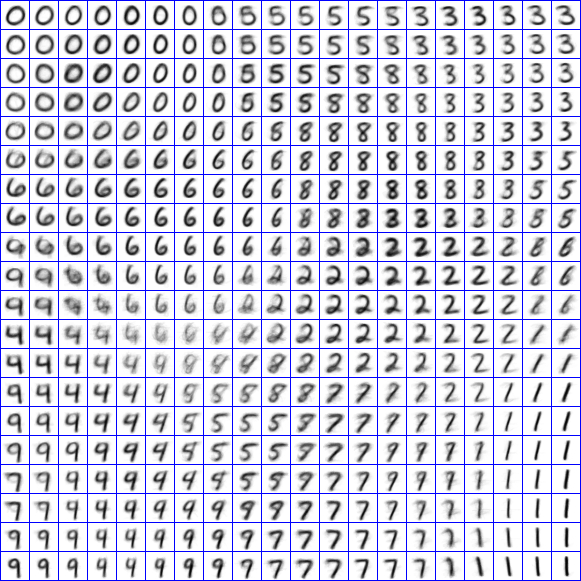
\includegraphics[width=0.5\textwidth]{digits.jpg}
\caption{Représentation de la base de données MNIST, images de chiffres écrits à main levées, par une SOM en deux dimensions. Une continuité est observée dans la forme des images lorsqu'on se déplace dans la carte~: le $0$ se transforme en $6$, etc.}
\label{fig:digits}
\end{figure}

\begin{figure}
    \centering
    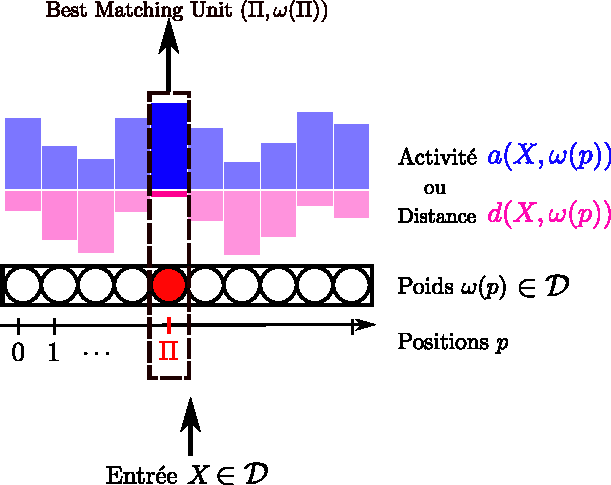
\includegraphics{SOM.pdf}
    \caption{Elements principaux composant une carte de Kohonen: une carte prend une entrée $X$, un ensemble d'unités de poids $\omega$ et indexées par une position $p$~; une activité $a$ ou une distance $d$ est calculée pour chaque unité par rapport à l'entrée. La Best Matching Unit, abrégée en BMU, est calculée comme l'unité d'activité maximale sur les positions (ou de distance minimale). Sa position est notée $\bmu$ et son poids est ainsi $\w(\bmu)$.  \label{fig:SOM}}
    \end{figure}
    

\subsection{Aspect topologique de la carte de Kohonen}

La carte de Kohonen se distingue d'autres algorithmes de quantification vectorielle par la topologie introduite par la carte dans l'ensemble des prototypes. Cette topologie dépend du voisinage utilisé par l'algorithme et de la dimension du support de la carte.
La plupart des implémentations de SOMs de la littérature utilisent comme support une grille en deux dimensions. L'indexation des n\oe{}uds est alors un ensemble de positions 2D. Des exemples de topologies en ligne et grilles sont présentées en figure~\ref{fig:topo}

En théorie, les cartes peuvent être une dimension (ligne), deux dimensions (grilles), ou de dimensions plus grandes. Les cartes peuvent aussi être des graphes de forme plus variable. 
En pratique, les grilles en deux dimensions sont les supports les plus couramment utilisés. Ces grilles permettent d'effectuer une réduction de dimension, tout en étant facile à visualiser sur un écran. Les cartes de dimensions supérieures sont très rarement utilisées dans la littérature. Le coût de l'algorithme d'apprentissage dépend en effet du nombre de neurones, et celui-ci augmente exponentiellement lorsqu'on augmente la dimension d'une carte de Kohonen. Les calculs deviennent alors rapidement coûteux.
Les cartes une dimension sont quant à elles limitées en termes de représentation des données et sont donc rarement utilisées en pratique. Cependant, elles se prêtent mieux à la représentation graphique et au développement de nouveaux modèles que les cartes 2D.
Les travaux conduits en \cite{cottrell_theoretical_2016,fort_soms_2006} apportent par exemple une formalisation mathématique de l'algorithme de Kohonen et prouvent la convergence de cartes une dimension. Les auteurs se heurtent cependant à la preuve de convergence pour des cartes en deux dimensions. Donc, les processus intervenant dans des cartes 1D sont déjà mathématiquement difficiles à formaliser, difficulté qui augmente avec les dimensions.
L'étude des cartes 1D a ainsi l'intérêt d'envisager un modèle simplifié dans le cadre de développement d'un nouveau modèle de SOM, ce que nous chercherons à faire dans cette thèse, avant de proposer une extension aux cartes 2D.

Les cartes de forme autre que des grilles 1D ou 2D sont moins couramment utilisées, mais peuvent présenter des avantages. Ainsi, des cartes structurées en arbre telles que développées en~\cite{koikkalainen_self-organizing_1990} permettant une recherche de BMU structurée. Certains modèles construisent une carte de Kohonen en ajoutant des n\oe{}uds au fur et à mesure de l'apprentissage, générant une carte de Kohonen sous forme d'un graphe construit par l'algorithme, par exemple en~\cite{alahakoon_dynamic_2000, yamaguchi_adaptive_2010}.

\begin{figure}
\centering
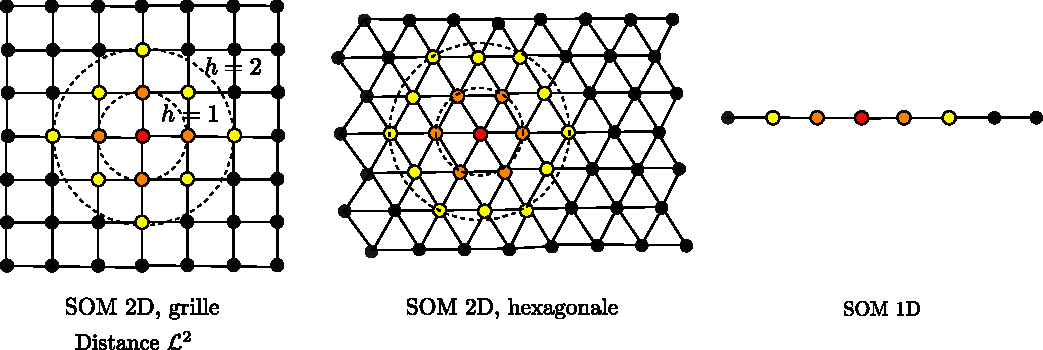
\includegraphics[width=0.8\textwidth]{soms_topologies}
\caption{Exemples de connexions dans le graphe support d'une SOM. Deux n\oe{}uds connectés sont ici à une distance de une unité dans la carte.
Les SOM en deux dimensions sont les plus communément utilisées dans la littérature, sous forme d'une grille ou d'une grille hexagonale. Les SOM une dimension sont également utilisées. \label{fig:topo}}

\end{figure}

\begin{figure}
\centering
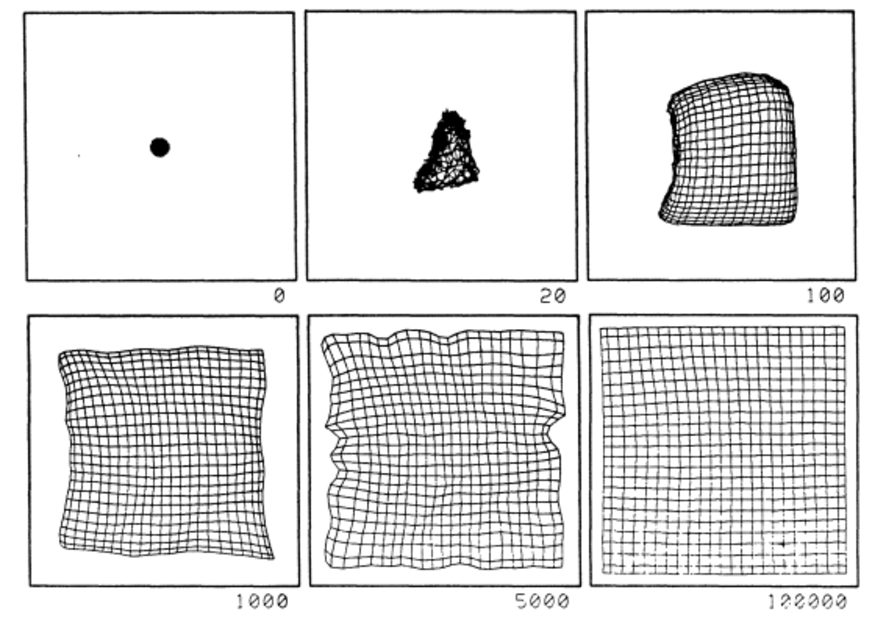
\includegraphics[width=0.7\textwidth]{som2d}
\caption{Dépliement d'une SOM 2D sur des données dans le plan $[0,1]^2$, tiré de~\cite{Kohonen1995SelfOrganizingM} \label{fig:som2d}}

\end{figure}

\begin{figure}
\centering
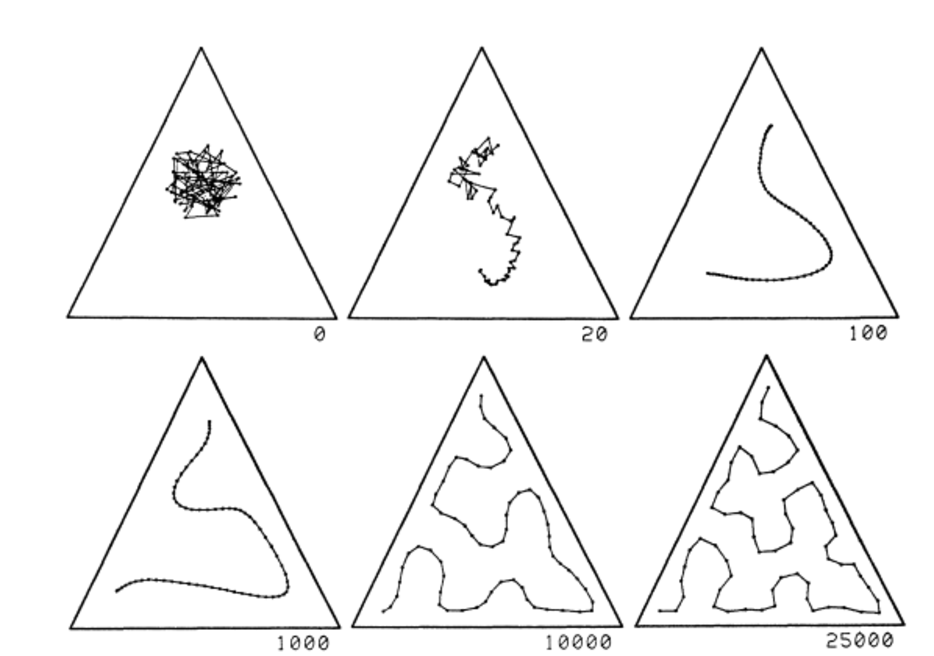
\includegraphics[width=0.7\textwidth]{som1d}
\caption{Dépliement d'une SOM 1D sur des données dans un triangle 2D, tiré de~\cite{Kohonen1995SelfOrganizingM}\label{fig:som1d}}

\end{figure}


\subsection{Inspiration biologique}

Le développement des cartes auto-organisatrices par Kohonen est initialement inspiré par les cartes topologiques observées dans les aires du cerveau. 
Le cerveau est cartographié en \emph{aires corticales} distinctes selon la fonction principale présumée de la zone du cortex correspondante.
Le découpage fonctionnel du cerveau fait apparaître des grandes catégories d'aires corticales. Certaines aires sont dites sensorielles, car elles reçoivent des entrées sensorielles via le thalamus. Certaines aires sont dites motrices et reliées aux muscles, via des structures sous corticales et permettent ainsi un contrôle moteur.
Enfin, des aires sont identifiées comme traitant des informations venant de plusieurs autres aires.
De nombreux travaux montrent la présence de cartes topologiquement ordonnées dans différentes aires du cortex cérébral: les neurones proches dans le substrat cortical réagissent à des stimuli proches. 
Un exemple est ainsi celui du cortex visuel V1, représenté en figure~\ref{fig:v1}. 
L'aire associée à l'audition présente aussi une organisation topographique \cite{Reale1980TonotopicOI}, ainsi que de nombreuses autres aires, directement sensorielles ou plus abstraites \cite{Kohonen1995SelfOrganizingM}. 
Une carte de Kohonen ne doit cependant pas être considérée comme une modélisation biologiquement plausible d'une aire du cortex cérébral, mais plutôt comme une adaptation au niveau computationnel d'un concept biologique, ici le concept d'organisation topologiquement correcte dans les cortex sensoriels, tel que le cortex visuel ou auditif.

\begin{figure}
\centering
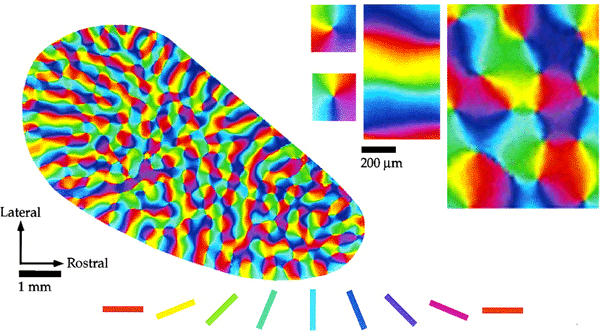
\includegraphics[width=0.6\textwidth]{v1.jpg}
\caption{Représentation des réponses du cortex visuel V1 à un stimulus visuel (bâtonnets d'orientations spatiales différentes). Les neurones répondant à une certaine orientation sont affichés de la même couleur. On observe une continuité entre les neurones proches dans le cortex et l'orientation à laquelle ils répondent. Cette propriété d'organisation est l'inspiration biologique des cartes de Kohonen.}
\label{fig:v1}
\end{figure}


Les aires du cerveau sont connectées entre elles. Notons que cette connectivité du cerveau peut-être étudiée de plusieurs points de vue~: d'un point de vue structurel, en se basant sur des éléments anatomiques ou fonctionnel.
Dans le cas fonctionnel, la connexion de deux aires est déduite de l'existence de dépendances statistiques entre l'activation des neurones des deux aires, observées par éléctroencéphalographie ou IRM fonctionnelle. Il faut noter cependant que ces observations traduisent une relation statistique et pas forcément une relation de cause à effet. 
La modélisation de la connectivité physique de ces aires à partir des observations reste donc l'objet de différentes théories cherchant à reproduire ces corrélations. 
Dans tous les cas, la présence d'aires distinctes communicantes fait l'objet d'un consensus.
Des modèles communs pour cette communication entre neurones sont par exemple la zone de convergence-divergence de Damasio (CDZ) \cite{damasio_time-locked_1989}, et le modèle de boucles de rée-ntrées de Edelmann \cite{Edelman1982GroupSA}.
La zone de convergence divergence suggère que certaines aires corticales servent d'aires associatives pour associer d'autres zones corticales prenant des modalités sensorielles en entrée. Ces aires associatives assemblent les signaux en provenance des zones sensorielles et les propagent vers d'autres zones. 
La théorie de la ré-entrée postule quant à elle des connexions directes et réciproques entre les neurones de différentes zones sensorielles ou non. Ces connexions sont à l'origine de la coactivation de neurones dans différentes cartes.
% Un tel traitement de l'information permettrait ainsi d'expliquer l'effet ventriloque \cite{Bonath2007NeuralBO}. Lors de cet effet, une activité apparaît dans les cortices visuel et auditif pour les neurones sensibles à l'emplacement exact de la source des stimuli dans chacune des modalités. Après quelques millisecondes, correspondant au temps de trajet de l'aire visuelle à l'aire auditive via les aires associatives, on observe une activité auditive pour les neurones sensibles à l'emplacement spatial de la source du stimulus visuel.

% Le modèle classique du cerveau proposé dans les années 60 [Jones and Powell, 1970] modélise le cortex comme un système de traitement hiérarchique et séquentiel de l'information. Les différents flux sensoriels seraient traités par des aires corticales dédiées, et leur mise en relation dans des aires associatives ui s'occuperaient de tâches de plus haut niveau. 
% Ces flux d'informations circuleraient dans les deux sens: une aire de plus haut niveau recoit des flux d'information montant d'une aire sensorielle, et l'aire sensorielle reçoit des flux d'information descendant des aires associatives. Ce modèle de connexion est par exemple modélisé en \cite{damasio_time-locked_1989}, travaux dans lesquels les zones associatives sont désignées par "zones de convergence-divergence".

% Cette vision hiérarchique historique du traitement cortical de l'information est cependant remise en question par d'autres observations biologiques. Ainsi, \cite{eckert_cross-modal_2008} suggère l'existence de connexions directes entre les aires sensorielles visuelles et auditives. Des théories telles que la réentrée suggère l'existence de neurones multimodaux au sein d'une aire sensorielle. Anatomiquement, de nombreuses connexions, dites bas niveau, entre les aires corticales dédiées au traitement d'une modalité sensorielles ont été mises en évidence chez différentes espèces, pour des aires à différents niveaux hiérarchiques de traitement de l'information(voir [Calvert and Thesen, 2004b, Cappe et al., 2009, Cappe and Barone, 2005, Foxe and Schroeder, 2005, Kayser and Logothetis, 2007, Macaluso, 2006, Schroeder et al., 2003, Schroeder and Foxe, 2005]).


La carte de Kohonen implémentant des concepts computationnels qu'on retrouve en biologie au niveau de l'aire cérébrale, nous pouvons chercher à pousser l'inspiration biologique d'une carte de Kohonen au niveau des connexions entre les aires cérébrales, se transcrivant par des connexions entre plusieurs cartes de Kohonen.
De la même façon qu'une carte n'est pas un modèle biologique, il s'agit plutôt de développer un modèle computationnel qui ne soit pas biologiquement plausible au niveau neuronal, mais dont la structure du traitement de l'information est inspirée de celle du cerveau, ici la présence de plusieurs aires connectées entre elles, modélisées par l'utilisation de plusieurs cartes de Kohonen en architecture.

\section{Architectures de cartes auto-organisatrices}

Plusieurs travaux dans la littérature informatique autour des SOMs cherchent ainsi à construire des architectures de cartes auto-organisatrices, que nous passons en revue dans cette section.
Nous abordons ces modèles d'un point de vue structurel en s'intéressant notamment à comment s'effectue l'interface entre les cartes dans chacun des modèles.

Il s'agit d'abord de différencier les architectures appliquées au traitement d'un problème particulier et les architectures génériques de cartes de Kohonen.
Pour résoudre un problème compliqué, une démarche courante est de le décomposer en sous-problèmes et de créer des algorithmes pour résoudre ces sous-problèmes. L'assemblage des résultats de chacun de ces sous-problèmes donne alors souvent une solution pour résoudre le problème général.
Nous différencions cette vision d'architecture appliquée de la notion d'architecture générique. 
Dans cette deuxième approche, on entend par modèle d'architecture le cadre de calcul sous-jacent au modèle, appliqué ou non, défini par ses règles de construction. Ce cadre est générique et utilisable sur n'importe quelles données d'application. C'est cette deuxième approche que nous étudions dans cette thèse. Nous nous concentrons particulièrement sur les architectures modulaires.
Le principe d'une architecture modulaire est d'assembler un nombre variable d'éléments de même type, des modules, dans une architecture. Ici les modules seront des cartes auto-organisatrices, dont le modèle a été adapté pour permettre la construction d'architectures.

\subsection{Méthode d'analyse}

L'étude des architectures développées dans les travaux précédents nous amènent à différencier les structures selon plusieurs aspects. Nous les classerons d'abord selon leur structure: hiérarchique et non-hiérarchique.
Nous analyserons dans ce cadre leur mode de communication et les attributs servant de vecteur de transmission d'information entre modules. Nous y ajouterons leurs différences lors de la séquence de mise à jour dans un contexte d'apprentissage.

\paragraph{Architectures hiérarchiques et non-hiérarchiques}

Nous distinguerons deux structures d'architectures de cartes~: les architectures \emph{hiérarchiques} et les architectures \emph{non-hiérarchiques}.
La structure d'une architecture de cartes auto-organisatrice peut se représenter comme un graphe orienté, dans lequel les n\oe{}uds correspondent à un module, c'est-à-dire une carte. Lorsque la carte B utilise des informations provenant de la carte A lors de son apprentissage, une arête de A vers B est présente dans le graphe. Ce graphe est le graphe de connexion de l'architecture.

Une architecture est dite hiérarchique lorsqu'il n'existe pas de cycle dans le graphe de connexions. Dans ce cas, les arêtes sont orientées dans le même sens et on peut définir des niveaux de cartes. Toutes les cartes d'un même niveau ne sont pas connectées entre elles, ont au moins une connexion arrivant du niveau précédent et/ou une connexion sortant vers le niveau suivant.
Une architecture est non-hiérarchique lorsqu'il existe au moins une boucle dans le graphe de connexions. Celle boucle peut être une connexion bidirectionnelle entre deux cartes ou une boucle comprennant plus de n\oe{}uds. Ces boucles implémentent des rétroactions entre les cartes de l'architecture.
Au sein des architectures non-hiérarchiques, nous verrons qu'il existe deux paradigmes que nous détaillerons dans la section correspondante~: les architectures centralisées et décentralisées.


Ces types d'architectures se ressemblent dans leur conception~: une architecture hiérarchique est ainsi un cas particulier d'architecture non-hiérarchique~; toute architecture non-hiérarchique est un cas particulier d'architecture décentralisée. Une architecture décentralisée est alors le modèle le plus générique d'architecture modulaire.
La construction d'une architecture plus générique amène des contraintes supplémentaires, notamment la gestion des rétroactions dans les méthodes de communication et d'apprentissage.
Nous classerons donc les modèles du plus spécifique au plus générique. Une architecture hiérarchique peut donc être construite à partir d'un modèle non-hiérarchique~; nous verrons en effet que les modèles hiérarchiques et non-hiérarchiques se rejoignent dans leur conception.

\begin{figure}
    \centering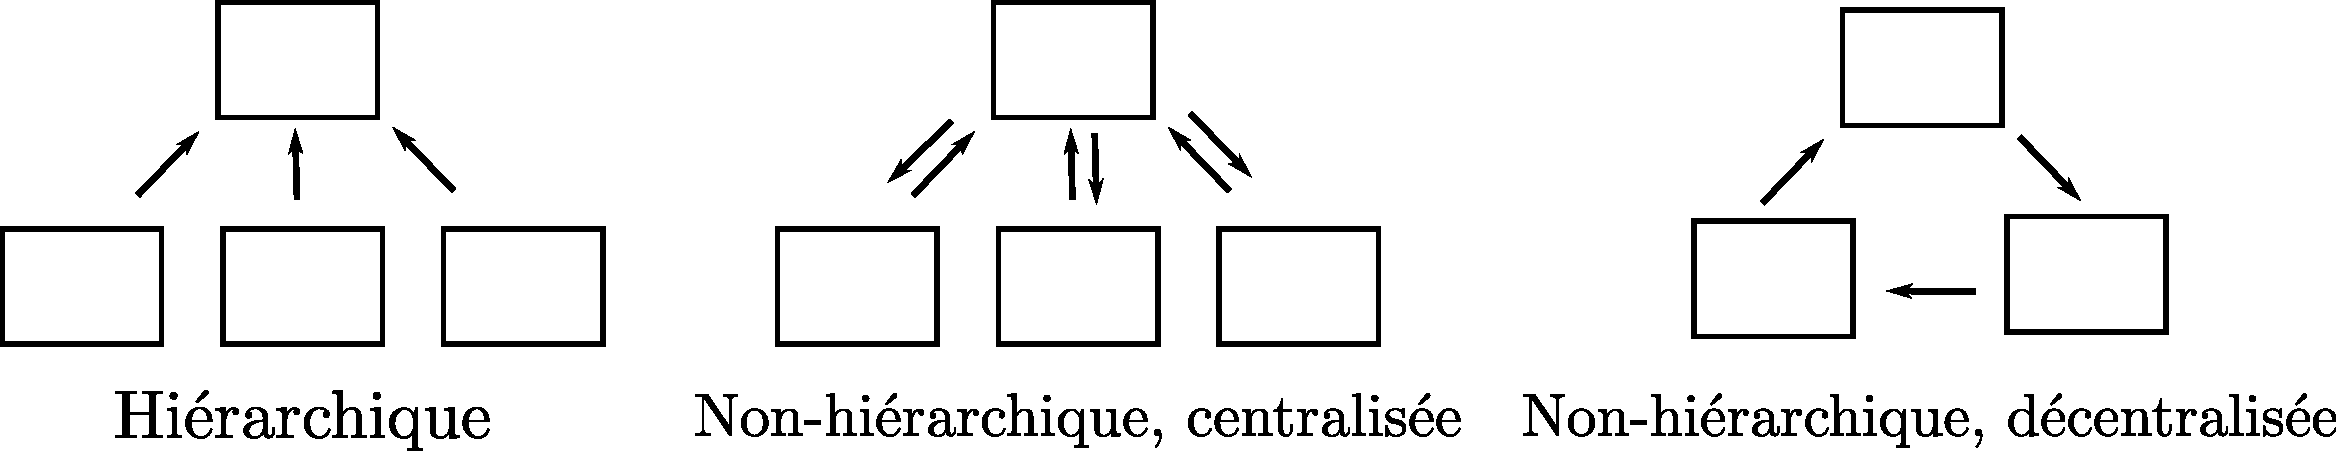
\includegraphics[width=0.8\textwidth]{structures_002.pdf}
    \caption{Exemples de connexions dans des architectures hiérarchiques et non-hiérarchiques centralisées et décentralisées. Un rectangle correspond à un module, ici une carte auto-organisatrice. \label{fig:graphe}}
    \end{figure}

\paragraph{Granularité du calcul et temporalité de l'apprentissage}

Pour chaque catégorie d'architecture, nous analyserons le mode de connexion entre cartes. Cette communication est réalisée soit par une surcouche algorithmique, soit est interne à l'organisation d'une carte.
Cette surcouche algorithmique se présente sous forme de sélection ou ajout de cartes pour l'apprentissage des données d'entrées. 
Nous présenterons des exemples de modèles de ce type dans le paragraphe suivant. La communication effectuée par une telle surcouche est alors globale à l'architecture.
La communication est interne à l'organisation d'une carte lorsque les données transmises sont directement prises en compte dans l'algorithme de mise à jour. Ainsi, les cartes ou les n\oe{}uds implémentant une telle communication prennent en tant qu'entrée des éléments de sortie des autres cartes, telles que la position du BMU, son poids ou une activité neuronale. La communication réalisée de cette manière est donc plutôt locale à une carte.
Au sein d'une méthode de connexion, les éléments transmis entre cartes varient. Certaines architectures utilisent ainsi la position du BMU, son poids, ou encore un ensemble d'activités de neurones d'une carte.


Enfin, la temporalité de l'algorithme de mise à jour de l'architecture peut se présenter de différentes façons. Nous distinguerons d'abord des architectures ayant une mise à jour séquentielle~: l'architecture peut être décomposée en groupes d'éléments indépendants, comme les niveaux d'une architecture hiérarchique. 
Un apprentissage complet est d'abord effectué sur un groupe avant de passer à l'apprentissage du groupes suivants. 
Les mises à jour peuvent au contraire être réalisées en une seule étape, lors de laquelle les éléments seront tous mis à jour en tenant en compte des dépendances. Dans ces cas, ces mises à jour peuvent être synchrones~: une itération d'apprentissage peut être définie de façon globale à toute l'architecture, lors de laquelle tous les éléments seront mis à jour au moins une fois. Les signaux lançant l'opération de mise à jour d'une carte sont régis par un processus extérieur aux cartes.
Les mises à jour asynchrones sont quant à elles effectuées seulement lorsqu'un signal déclenchant la mise à jour est transmis à un élément (carte ou neurone). C'est notamment le cas dans les réseaux de neurones impulsionnels, dans lequel les paramètres d'un neurone sont mis à jour seulement lorsqu'une impulsion lui parvient. Ce mode de mise à jour repose encore plus sur une notion de calcul local.

Nous verrons ainsi que les modèles existants d'architecture de cartes se placent dans ces quelques catégories. Cette taxonomie générale est décrite en figure~\ref{fig:structure}.
L'analyse de ces modèles nous permet de nous situer dans la littérature et d'émettre des hypothèses concernant les comportements attendus d'un tel modèle et ainsi de guider les expériences que nous effectuerons.

% \begin{table}
%     \begin{tabular}{l|llllllllllll}
%         \toprule
%         \multicolumn{1}{l|}{Structure} & \multicolumn{6}{c|}{Hiérarchique} &  \multicolumn{6}{c}{Non-Hiérarchique} \\
%        \midrule
%        \multicolumn{1}{l|}{Mode de transmission}& \multicolumn{2}{l|}{Par sélection} & \multicolumn{10}{l}{Transmission de représentation interne}\\
%        \multicolumn{1}{l|}{\emph{Granularité}} & \multicolumn{2}{l|}{\emph{Surcouche Algorithmique}} & \multicolumn{10}{c}{\emph{Locale à une carte}}\\
%         \midrule
%         \multicolumn{1}{l|}{Mises à jour \hfill} & \multicolumn{6}{l|}{Séquentielles \hfill} &  \multicolumn{4}{l|}{Synchrones} &  \multicolumn{2}{l}{(Asynchrones)} \\
%         \midrule
%         Elements transmis & \multicolumn{12}{l}{Position du BMU, poids du BMU, activités ...}
%     \end{tabular}
% \end{table}

\begin{figure}
\centering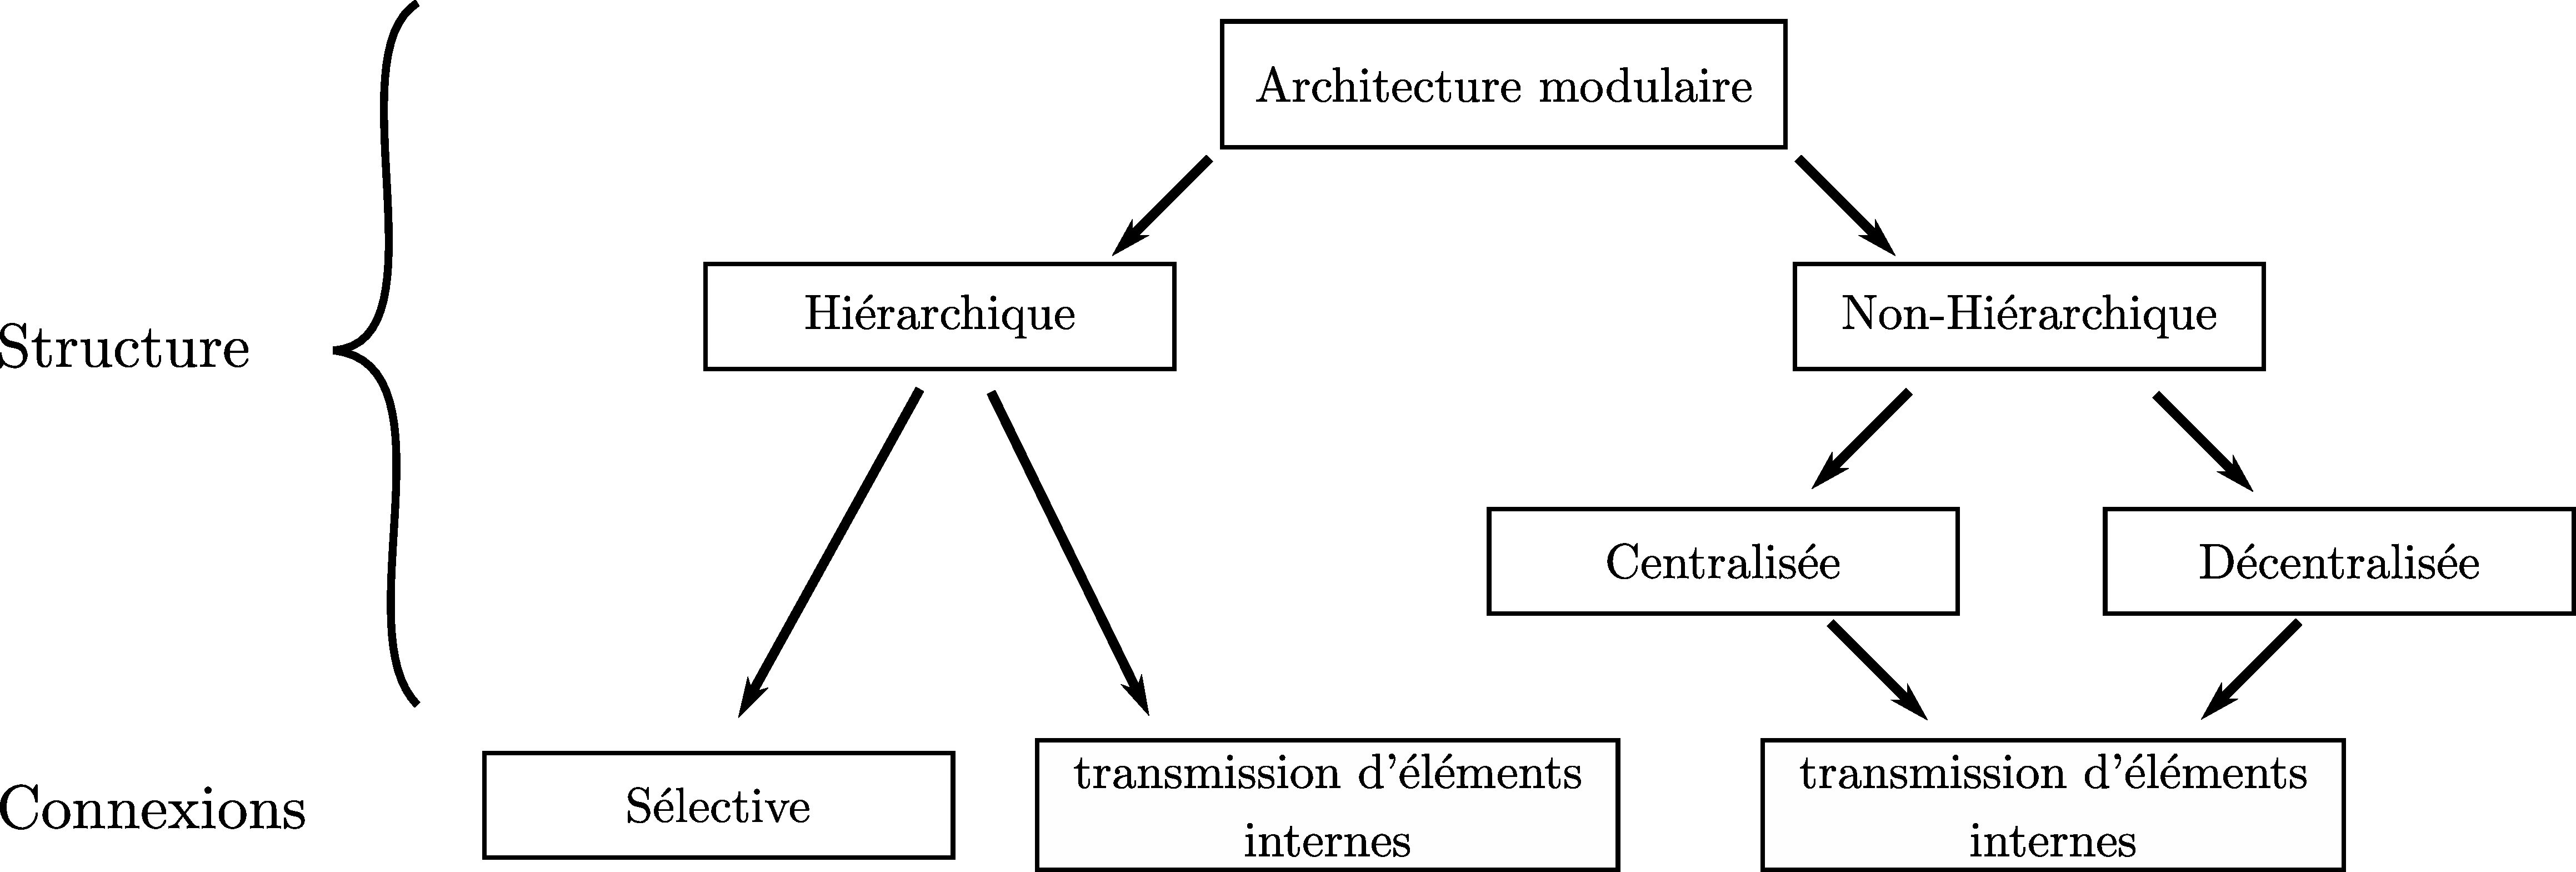
\includegraphics[width=\textwidth]{structures.pdf}
\caption{Taxonomie des architectures de cartes présentées dans ce chapitre. Nous analyserons comment leurs caractéristiques structurelles: hiérarchiques ou non-hiérarchiques, centralisées, décentralisées, façonne leur comportement d'apprentissage. Nous analyserons également leur interface de communication. Nous n'avons pas relevé d'architecture non-hiérarchique s'appuyant sur le principe de sélection, car ce principe est fondamentalement hiérarchique. \label{fig:taxo}}
\end{figure}



\subsection{Architectures hiérarchiques de cartes}

Des travaux portant sur les architectures de cartes ont été conduits dès la création du modèle de carte de Kohonen.
Nous avons divisés celles-ci en deux catégories. 
La première est celle des architectures sélectives, dans laquelle le premier niveau est généralement une carte seule et le nombre de cartes augmente au fur et à mesure des niveaux. Toutes les cartes ont pour entrée des données du même ensemble et la transmission de données entre carte repose sur la sélection d'une carte d'un niveau en fonction de l'activation du premier niveau. 
L'autre catégorie est celle des architectures par transmission de représentation. Dans ce cas, les cartes du deuxième niveau prennent en entrée la sortie du premier niveau et non les données d'entrées. Le nombre de cartes diminue alors au parcours des niveaux le dernier niveau formant une représentation plus abstraite de l'espace d'entrée.
Nous présenterons les différents modèles dans le formalisme introduit en section~\ref{sec:som001}. Par facilité de représentations, les schémas des architectures sont présentés avec des cartes en une dimension. Cependant, toutes les architectures présentées utilisent des cartes en deux dimensions, parfois plus.
% La mise à jour des cartes dans toutes ces architectures est effectuée séquentiellement~: le processus d'apprentissage est réalisé du début à la fin sur l'ensemble des cartes, non connectées, du premier niveau. Une fois ce niveau organisé, une nouvelle phase d'apprentissage est entièrement réalisée sur le deuxième niveau, en prenant en compte les sorties du premier, etc.
\subsubsection{Architecture hiérarchique par sélection}

%TODO Phrase d'intro
Prenons en exemple l'architecture sélective \cite{barbalho_hierarchical_2001} en figure \ref{fig:hsom_selective}. Ce modèle est décliné en une version dynamique dans laquelle les paramètres des cartes dépendent des données, en \cite{Costa2016ANS}.
Le premier niveau de cette architecture est une carte classique, prenant des données $X$ dans un espace d'entrée $\mathcal{D}$.
La première étape de l'apprentissage est une étape d'apprentissage complet de la carte du premier niveau.
Après apprentissage du premier niveau, le second niveau est composé de plusieurs cartes~; chacune de ces cartes est associée à un des n\oe{}uds de la première.
Pour la deuxième phase de l'apprentissage, les données d'entrées sont réparties en sous-ensemble, tel que chaque sous-ensemble $\mathcal{D}_i$ est l'ensemble des entrées $X_t$ ayant $i$ pour position du BMU associé à l'entrée. Cette répartition est effectuée lors d'un passage de test des entrées, pendant lequel les poids ne sont pas mis à jour.
Chaque carte $i$ du deuxième niveau est alors entrainées sur son espace $\mathcal{D_i}$; les cartes du premier niveau n'étant plus mises à jour.
Dans la version de \cite{barbalho_hierarchical_2001}, l'architecture de carte est définie à l'avance. Dans la version dynamique, l'ajout de niveau hiérarchique est soumis à la condition que la carte enfant d'un n\oe{}ud doit permettre de réduire d'au moins 20\% l'erreur de quantification sur le sous-espace associé. Autrement dit, si tous les points ayant le même BMU sont a proximité immédiate du poids du BMU, aucune carte n'est générée pour le niveau suivant. Dans cette version dynamique, les auteurs font également varier la taille de la carte d'un niveau en fonction de la cardinalité du sous-ensemble de données utilisé pour l'apprentissage de cette carte.
L'ensemble des prototypes des cartes, non seulement ceux du dernier niveau, forment alors une cartographie plus précise de l'espace d'entrée~: l'erreur de quantification vectorielle y est plus faible.

Ce processus est sélectif dans la mesure ou chaque carte se voit sélectionnée pour l'apprentissage d'une entrée en fonction de l'état du niveau précédent. Dans ces travaux, la position du BMU est utilisée comme information pour la sélection. 
Dans ce type d'architecture, c'est un processus extérieur aux cartes qui permet de sélectionner la carte du niveau suivant, ou de créer ou non des cartes à ajouter à l'architecture. L'algorithme de mise à jour des poids de l'architecture est ainsi sous la dépendance d'un processus global.

%TODO AUTRES
Ce procédé de sélection se retrouve dans de nombreux travaux. 
Les auteurs de \cite{zhao_stacked_2015} développent par exemple un ensemble de cartes et leur règles de communication spécifiquement adapté à de la détection d'arrière plan dans des séquences.
\cite{miikkulainen_script_1992} traite des données à structure hiérarchiques: leur architecture est spécifique à
Ce procédé sélectif est retrouvé dans d'autres architectures telles que \cite{suganthan_pattern_2001}, \cite{miikkulainen_script_1992} pour de la classification de phrases, \cite{dittenbach_growing_2000,ordonez_hierarchical_2010}.
En terme d'application, les architectures sélectives permettent à chacune des cartes de se spécialiser sur une partie de l'espace d'entrée. 
En général, le premier niveau seul est une représentation moins précise de l'espace d'entrée. L'augmentation et la séparation des cartes dans les niveaux supérieurs permet une meilleure précision de quantification vectorielle du modèle appris.


%TODO CONCLUSION : Ca nous intéresse moins, mais il semblait important de remarquer l'existence de ce type d'architecture pour bien nous en différencier. On peut noter aussi que les BMUs, 
L'aspect global du processus de connexion des cartes dans ce type d'architecture nous intéresse moins d'un point de vue modulaire. Ces architectures sont plutôt des agrégations de cartes de Kohonen dont on étudie les


\begin{figure}
    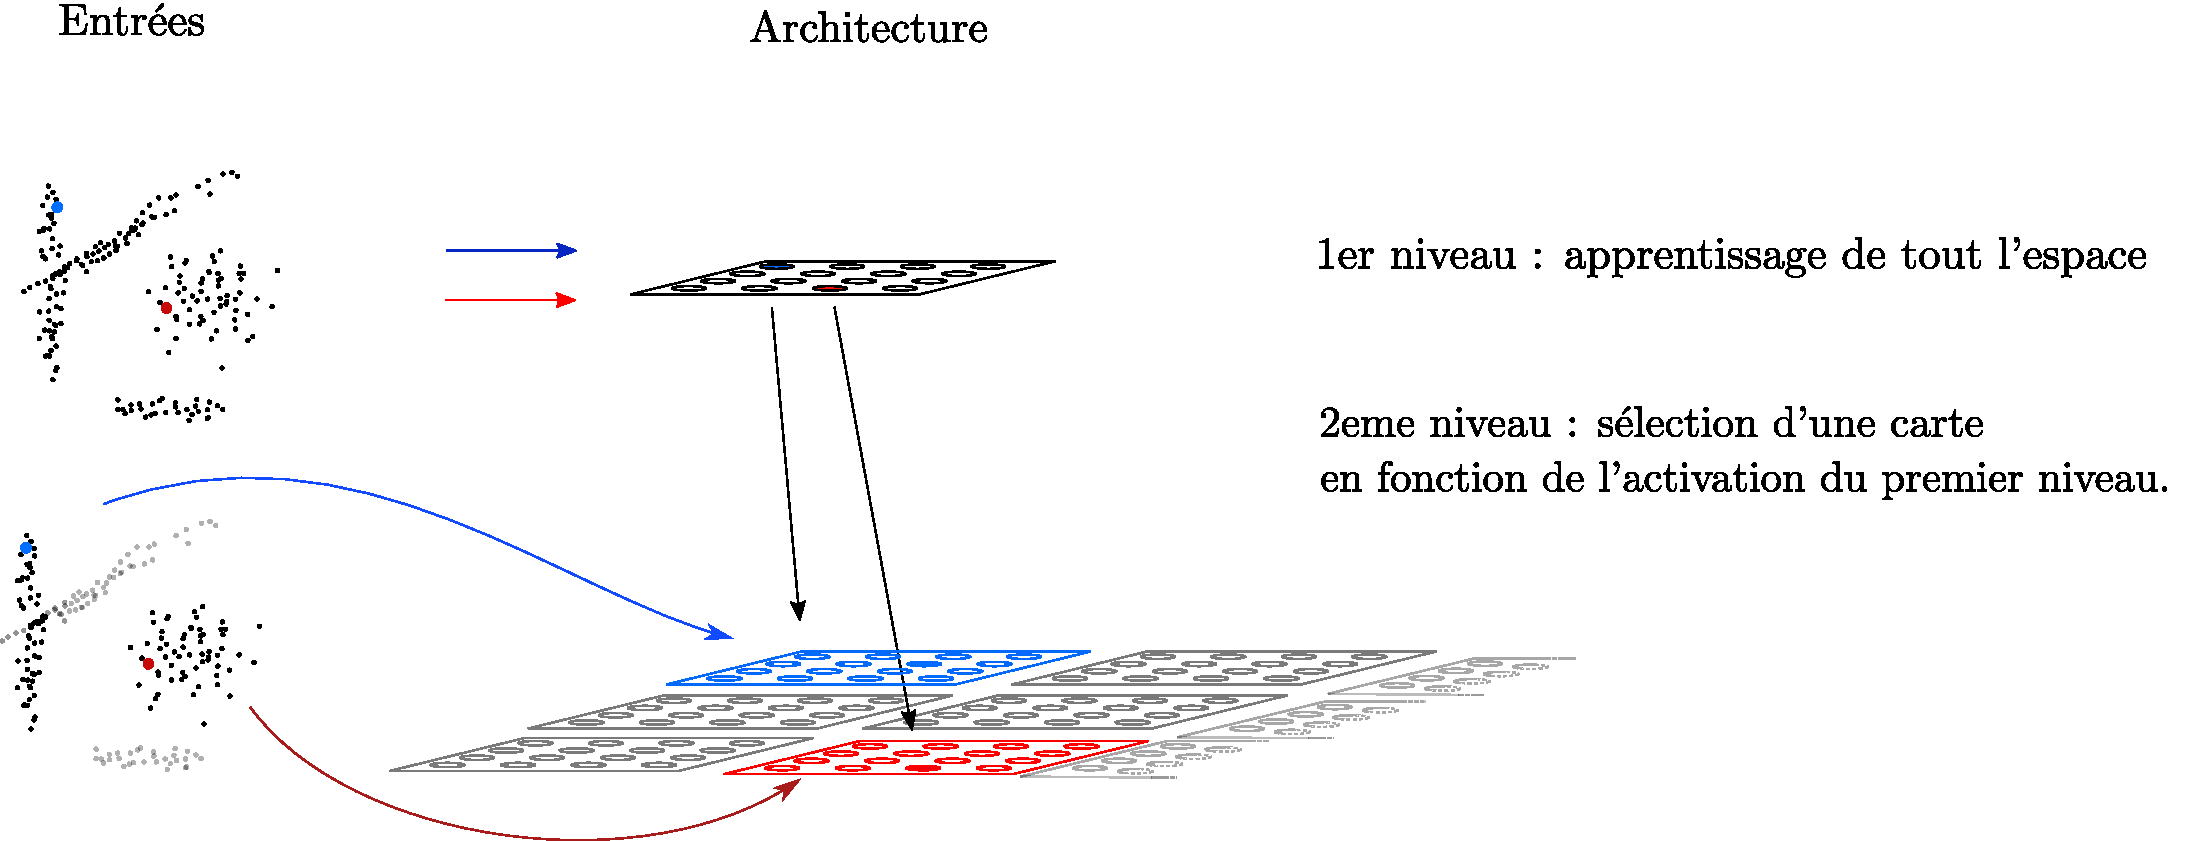
\includegraphics[width=\textwidth]{HSOM_selective.pdf}
    \caption{Exemple d'architecture hiérarchique sélective. La carte du premier niveau est entraînée sur tout l'espace d'entrée. Après apprentissage, la carte permet de filtrer les entrées pour les renvoyer vers une carte du niveau suivant. Dans cet exemple, la position du BMU de la carte du niveau 1 permet de sélectionner une carte du niveau 2, comme c'est le cas en \cite{barbalho_hierarchical_2001}. 
    L'entrée permet d'entraîner une carte du deuxième niveau. Chacune des cartes du niveau 2 apprend alors sur un sous-espace d'entrée. La carte $M$ est représentée sur les données d'entrée (disposition exemple, non générée par une simulation). Le sous espace $\mathcal{D}_1-$ lié au BMU à la position $1$ alimente alors une carte du deuxième niveau $M_1$.
    \label{fig:hsom_selective}}
\end{figure}


\subsubsection{Architectures hiérarchiques par transmission de représentation intermédiaire}

Certaines architectures implémentent une interface entre cartes gérée directement au niveau du processus d'auto-organisation de la carte.
Cette gestion des connexions qui était collective dans les architectures sélectives devient locale~: aucune surcouche algorithmique globale à l'architecture n'intervient dans les tâches de transmission d'information. Notons que la gestion des itérations peut rester globale à l'architecture.
Ce traitement local de l'information se rapproche plus de l'aspect modulaire que nous étudions.

Contrairement aux architectures par sélection, la deuxième couche de carte ne prend plus comme entrée un élément de l'espace d'entrée de l'architecture, mais travaille sur des éléments des cartes des couches précédentes, tels que la position, le poids du BMU ou une intensité d'activité neuronale. 
Ces éléments sont une représentation latente intermédiaire de l'entrée, transmise à la couche supérieure. Les niveaux supérieurs de ce type d'architecture ont généralement moins de cartes que les premiers niveaux et peuvent être considérés comme traitant l'information à un niveau plus abstrait que les cartes du premier niveau.

\paragraph*{Transmission du BMU}
L'architecture  HSOM \cite{lampinen_clustering_1992}, proposé dès 1992 et inspirant ensuite de nombreux modèles d'architecture hiérarchiques, est composée de deux cartes~: une carte apprenant sur des entrées $\inpx$, et une carte prenant comme entrée la position du BMU $\bmu$ de la première carte~; cette architecture est illustrée en figure~\ref{fig:hsom}. 

La représentation intermédiaire transmise aux cartes du niveau suivant est ici la position du BMU.
Comme les cartes s'organisent de façon à conserver les distances dans l'espace d'entrée au sein de la carte, deux éléments faisant partie d'un même groupe de données (cluster) auront des BMUs proches dans la première carte~; par conséquent, leurs BMUs dans la seconde carte le seront également. 
Les auteurs notent que l'architecture HSOM modifie les classes de données définies par une SOM. Une SOM classique utilisera 
Le fait d'utiliser deux SOMs permet ainsi d'extraire une représentation différente que celle extraite par une SOM classique.

D'autres travaux par la suite implémentent des modèles similaires transmettant la position du BMU entre cartes, sur des architectures comportant plus de cartes que HSOM, tel que \cite{hagenauer_hierarchical_2013, Paplinski2005MultimodalFS}. Dans leurs travaux, les auteurs implémentent une architecture en arbre. Une carte d'un niveau reçoit alors un vecteur de position de BMUs du niveau inférieur en tant qu'entrée.

Cette information transmise doit permettre de véhiculer un maximum d'information entre cartes, tout en étant interprétable par les autres cartes. Les architectures HSOM et ses dérivées utilisent la position du BMU en tant que représentation.
Par le choix de la position du BMU comme vecteur de transmission d'information, les auteurs de HSOM exploitent totalement l'aspect topologique qu'offrent les cartes de Kohonen. Cette information est par ailleurs relative à une carte et non un type d'entrée ce qui en fait une interface très générique. Enfin, il s'agit d'une position 1D ou 2D, donc une information légère.

Le terme de Deep SOM est souvent rencontré lorsqu'on s'intéresse aux architectures de cartes auto-organisatrices.
Les travaux se décrivant par ces termes implémentent des structures qui rejoignent celles présentées précédemment, mais puisent leur inspiration des réseaux de neurones profonds (\emph{Deep Learning}), ayant notamment connu leur essor avec les réseaux convolutionnels permettant l'apprentissage supervisé d'images \cite{lecun_deep_2015}.
Par analogie avec ces réseaux convolutionnels, les réseaux présentés comme Deep SOM s'intéressent à l'apprentissage d'images par des SOMs. 
La façon d'associer ces cartes en architecture rejoint néanmoins les SOMs hiérarchiques par transmission de représentation par leur mécanismes de transmission d'information.

Par exemple, le modèle D-SOM introduit en \cite{Liu2015DeepSM} et développé \cite{wickramasinghe_deep_2019}  est illustré en figure~\ref{fig:dsom}.
Le but d'une telle architecture est de classifier des images fournies en entrée de l'architecture.
Une fenêtre est déplacée sur l'image d'entrée et chaque imagette nourrit une carte d'une première couche, donnant $N_{maps}  \times N_{maps}$ positions de BMU $j_{p,q}$. Ces positions représentées comme des valeurs en une dimension sont assemblées en une image intermédiaire, chaque pixel prenant la valeur du BMU de la carte correspondante. Une deuxième étape de fenêtrage peut alors être appliquée sur cette image, et ainsi de suite. La dernière couche du réseau est composée d'une SOM qui effectue alors la tache de classification de l'image intermédiaire, vue comme une représentation abstraite  de l'entrée.
L'interface entre les couches de cartes est créée à partir des BMUs des SOMs: ce modèle de transmission rejoint ceux présentés précédemment. La différence vient seulement au niveau du prétraitement de l'entrée image, décomposée en imagette.
Les auteurs montrent que ce modèle est meilleur qu'une SOM classique dans des taches de classification sur MNIST~; les couches supérieures apportent un niveau d'abstraction tandis que les couches inférieures apprennent les motifs.
En\cite{nawaratne_hierarchical_2020-1}, les auteurs utilisent des cartes hiérarchiques pour la classification de données spatio-temporelles. Leur modèle est composé d'un premier niveau de deux cartes, dont l'une quantifie les 
La transmission de la posi


\paragraph*{Transmission du poids du BMU}

D'autres travaux, tels que ceux conduits en \cite{wang_comparisonal_2007, gunes_kayacik_hierarchical_2007} utilisent plutôt le poids du BMU comme  vecteur de transmission d'information.
Ainsi, \cite{dozono_convolutional_2016} décomposent l'image d'entrée en imagettes qui sont utilisées en tant qu'entrées d'une couche de cartes. Après apprentissage de cette couche, l'image est reconstruite grâce aux poids des BMU, puis décomposée en imagettes de tailles différentes pour être soumise à la deuxième couche de carte.
\cite{mici_self-organizing_2018} s'appuient sur des cartes hiérarchiques pour effectuer de la fusion de données spatio-temporelles. Les auteurs de ces travaux utilisent la position du BMU pour les sorties des cartes temporelles et son poids pour la sortie de la carte spatiale.

Ainsi \cite{hankins_somnet_2018,aly_deep_2020,sakkari_convolutional_2020,dozono_convolutional_2016,nawaratne_hierarchical_2020-1,mici_self-organizing_2018} et sont présentés comme des "SOMs convolutionnelles".

\begin{figure}
    \centering
    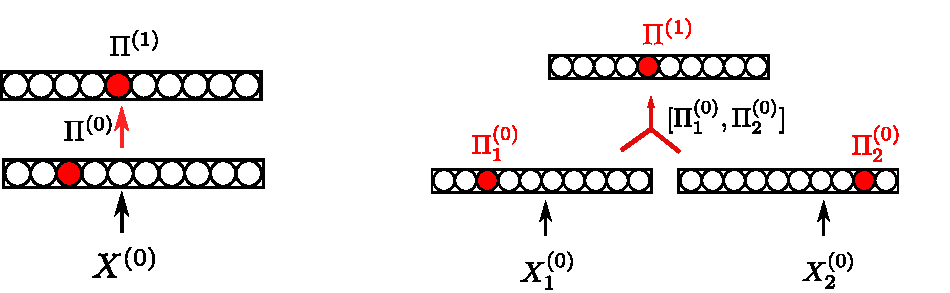
\includegraphics[width=\textwidth]{HSOM.pdf}
    \caption{Deux exemples d'architectures basées sur HSOM. A gauche, le modèle HSOM original proposé en \cite{lampinen_clustering_1992}. L'apprentissage des positions du BMU de la première couche par la seconde permet de mieux détecter les ensembles de données, dans une tâche de clustering. La deuxième couche est vue comme un niveau plus abstrait que la première. A droite, une version de HSOM à plus de cartes proposée en \cite{hagenauer_hierarchical_2013} permettant de faire du clustering sur des données multimodales: spatiales $X_1$ et temporelles $X_2$
    \label{fig:hsom}}
\end{figure}

\begin{figure}
    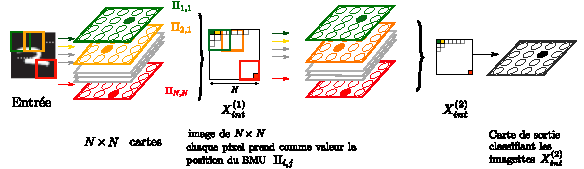
\includegraphics[width=\textwidth]{DSOM.pdf}
    \caption{Architecture DSOM de SOM "convolutionnelle" \cite{liu_deep_2015}. Les auteurs utilisent les positions des BMUs de la couche de carte $j_{p,q}$ comme valeurs d'entrée pour les couches suivantes, dans la lignée de HSOM \cite{lampinen_clustering_1992}. Les couches sont entraînées les unes après les autres. Cette architecture est \emph{feedforward} et \emph{hiérarchique} par transmission de représentation intermédiaire. \label{fig:dsom}}
\end{figure}

Toutes les architectures présentées ici, comme pour les architectures sélectives, sont ascendantes dans leur mise à jour~: chacune des couches de cartes sont entraînées les unes après les autres. 
Ces travaux sont appliqués à des tâches de classification qu'on pourrait aussi réaliser avec une SOM classique.
Les motivations pour utiliser une architecture plutôt qu'une SOM est d'abord le fait la couche finale du réseau possède de meilleures performances en termes de classification que si on avait utilisé une SOM simple.
D'autre part, la transmission d'une représentation interne aux carte au sein de l'architecture permet la fusion de données multimodales, comme proposé en \cite{mici_self-organizing_2018} et \cite{nawaratne_hierarchical_2020-1}. L'architecture permet alors de quantifier chaque modalité et d'en extraire une représentation interne. Toutes ces représentations sont homogènes et leur assemblage en tant qu'entrée d'une carte devient logique.


\subsubsection{Discussion}

Nous avons donc distingué deux catégories d'architectures hiérarchiques en s'appuyant sur le mode de connexion entre cartes dans l'algorithme de mise à jour. 
Le premier mode repose sur la sélection d'une carte du niveau supérieur en s'appuyant sur la réponse des cartes du niveau courant à une entrée, afin de transmettre cette entrée à la carte supérieure. Ce mode de transmission permet de créer un ensemble de cartes s'organisant sur un même espace d'entrée, laissant plus de possibilités au dépliement des cartes qu'une SOM classique. Ces types d'architectures permettent notamment d'améliorer la qualité de la quantification vectorielle générée par une SOM classique et d'ajouter des n\oe{}uds de façon peu couteuse. Le mode de transmission par sélection s'appuie sur une surcouche algorithmique aux cartes, qui analyse la sortie d'une carte et dirige l'entrée vers une aute carte

Le second mode de connexion repose sur la modification du principe de calcul d'activité et de mise à jour d'une carte pour prendre en compte les éléments de réponse d'une autre carte, par exemple en ajoutant cet élement de réponse en tant qu'entrée secondaire d'une carte.
Ce mode de connexion est intégré au processus d'auto-organisation et non une couche algorithmique supplémentaire comme les architectures par sélection, ce qui localise le traitement des connexions à l'échelle d'une carte. 
Cette méthode de construction d'architecture s'appuie sur la transmission d'une représentation de l'entrée interne entre cartes.
Ce type de connexions nous intéresse d'un point de vue modulaire : il autorise en effet l'ajout de modules à une architecture sans avoir à modifier toute la structure de l'architecture, ce qui est un des éléments de définition d'un système modulaire.
Nous verrons plus loin que les architectures non-hiérarchiques s'appuient toutes sur ce mode de transmission.
Nous avons relevé au sein des architectures hiérarchiques deux représentations internes majoritairement utilisées comme information transmise: la position du BMU ou le poids du BMU. La position du BMU est une représentation qui nous intéresse particulièrement, exploitant totalement l'aspect topologique d'une carte auto-organisatrice, de dimension faible et homogène entre cartes. Il permet aussi d'extraire une représentation abstraite de l'entrée, ce qui est le but recherché d'une architecture, par exemple dans le cas de la classification de données multimodales.
Le poids du BMU est moins spécifique à une carte de Kohonen, peut-être de dimension élevée et donc plus coûteux en terme de calcul dans une carte. Enfin, si les cartes de l'architecture prennent des entrées dans des espaces différents, cette représentation n'est pas homogène. Nous reviendrons sur ces modes de représentations en analysant les architectures non-hiérarchiques. Contentons nous de noter que la position du BMU est l'information principalement utilisée dans les architectures hiérarchiques.

Qu'elles soient sélectives ou par transmission de représentation, toutes les architectures relevées ici ont une séquence de mise à jour ascendante~: les cartes du premier niveau sont dépliées lors d'une première phase d'apprentissage. Une fois ces cartes dépliées, la deuxième couche est apprise à partir de la première lors d'une deuxième phase, lors de laquelle le premier niveau n'est plus mis à jour.
Le champ d'application des architectures hiérarchiques est le même qu'une SOM classique~: quantification vectorielle et classification.
Dans les deux cas, il s'agit d'améliorer les performances sur une tâche de quantification vectorielle ou classification pouvant être réalisée par une SOM. Par exemple, les SOMs par sélection permettent de mieux occuper l'espace d'entrée \cite{barbalho_hierarchical_2001} ou de prendre en compte l'aspect hiérarchique des entrées \cite{miikkulainen}, améliorant ainsi la quantification vectorielle. Les SOMs par transmission de représentation permettent de mieux isoler les clusters de données qu'une SOM classique \cite{lampinen_clustering_1992} ou d'effectuer une classification de données multimodales \cite{mici_self-organizing_2018}.
Nous pouvons donc considérer ces architectures comme des améliorations de carte auto-organisatrices sur des applications spécifiques.
Elles n'ont pas la capacité de faire d'autres types de calcul que ceux originalement réalisés dans une SOM.
L'aspect uniquement ascendant en est la cause~: les cartes de l'architecture agissent comme des filtres intermédiaires de l'information donnée en entrée, mais seule la couche finale est considérée en sortie de l'architecture : cette couche finale reste une carte auto-organisatrice classique, apprenant simplement sur des entrées filtrées.
% Le lecteur peut se référer à \cite{johnsson_spatial_2012} pour une revue des SOM hiérarchiques sous un angle plus appliqué.
Dans une volonté d'étudier une architecture proposant des comportements de calcul différents d'une SOM classique, notre attention se portera donc sur les architectures comportant des boucles de rétroaction~: les architectures non-hiérarchiques.
Ces architectures permettent de diversifier les comportements d'apprentissage qu'il est possible d'obtenir avec des SOMs en apportant un aspect dynamique au système par les rétroactions. Notons cependant qu'une architecture hiérarchique est un cas particulier d'architecture non-hiérarchiques~: les modèles que nous allons étudier en partie suivantes pourraient donc aussi être utilisés dans un cadre hiérarchique.


% C'est l'avenement du deep learning qui a poussé à créer des archi de SOMs. De la meme facon que les réseaux profonds ont étendu les capacités d'apprentissage du perceptron, les couhes de SOM montrent la meme ppté.
% Est-ce que la recherche actuelle sur l'apprentissage non supervisé poussera à remettre les SOM au gout du jour ? Est-ce qu'on ne fait pas de deep som, simplement parce que les outils n'ont pas été développés comme ceux du deep learning ? L'aspect non linéaire d'une SOM peut pourtant etre prometteuse dans ce cadre d'applis.
% Il s'agit par contre d'archiectures completement feed forward: on ne peut pas vraiment parler d'archi modulaires. Les couches sont apprises les unes après les autres.
% On fera référence à ce type d'archis comme des archis hiérarchiques.
% ces arhcitectures montrent des capacités d'apprentissage de motifs à plus grande echelle qu'une carte simple.

% \begin{itemize}
%     \item Historique de l'assemblage des SOMs en architectures feedforward ? 
%     \item Quels sont les avantages apportés par les deep SOMs par rapport à des Soms classiques
%     \item Quels sont les avantages des deep SOM par rapport aux réseaux de deep Learning 
%     \item Pourquoi ne sont elles pas plus utilisées maintenant ?
% \end{itemize}

\subsection{Architectures non-hiérarchiques de cartes auto-organisatrices}

Les architectures non-hiérarchiques de SOMs sont des architectures comportant plusieurs cartes communiquant entre elles et dont le schéma de connexion comporte des boucles de rétroaction~: une carte A reçoit de l'information d'une carte B, qui elle-même reçoit de l'information de la carte A.
% Ces architectures sont souvent proposées par une motivation d'inspiration biologique, en s'appuyant sur les théories mentionnées précédemment de la réentrée \cite{Edelman1982GroupSA} et des zones de convergence-divergence (CDZ) \cite{damasio_time-locked_1989}.
L'assemblage de réseaux de neurones en architecture fait l'objet de plus nombreux travaux dans le domaine des neurosciences computationnelles. Nous ne détaillerons pas ces travaux ici, nous intéressant spécifiquement aux modèles computationnels destinés à être appliqués en informatique et non modélisant finement la biologie.
Un inventaire des architectures de cartes non-hiérarchiques est ainsi assez ardu dans la mesure ou ces modèles sont développés dans le contexte des neurosciences computationnelles ou de la robotique cognitive et cherchent à modéliser les aires cérébrales. 
Nous chercherons à faire une revue de ces modèle d'un point de vue du calcul, tout en se positionnant à l'intersection des domaines précédemment évoqués.

Nous avons pu distinguer deux classes structures d'architectures non-hiérarchiques dans les travaux réalisés jusqu'a présent.
Certaines architectures comportent des cartes sensorielles qui sont reliées via des cartes associatives ne prenant pas d'entrées sensorielles, mais seulement des éléments de connexion interne. Ces architectures sont \emph{centralisées} dans la mesure ou ces cartes associatives centralisent l'information  montant des cartes sensorielles et la redistribuent. Ces architectures centralisées sont souvent désignées par leurs auteurs comme hiérarchiques~: en effet, les cartes associatives forment un niveau d'apprentissage différent des cartes sensorielles, apportant une hiérarchie dans l'apprentissage. Nous les classons ici dans la catégorie non-hiérarchique. Bien que des niveaux de cartes peuvent être isolés dans ces architectures, les connexions entre les cartes de deux niveaux sont bidirectionnelles, la carte associative étant à l'origine de l'activation de cartes sensorielles, et réciproquement.
Nous les différencions ainsi des cartes hiérarchiques feed-forward que nous avons listé au paragraphe précédent.
Le second type d'architectures non-hiérarchiques sont celles utilisant des connexions directes entre cartes sensorielles. Ces architectures sont \emph{décentralisées}~: il n'existe pas de module par lequel toute l'information transite.

Toutes ces architectures non-hiérarchiques ont en commun leur champ d'application~: contrairement aux architectures hiérarchiques feed-forward qui cherchent à améliorer les performances de classification ou de \emph{clustering} d'une SOM classique, les SOM non-hiérarchiques que nous avons relevées dans la littérature sont plutôt appliquées à des tâches de \emph{mémoire associative} sur des données \emph{multimodales}. 
Plus généralement, tous les modèles que nous présenterons cherchent à répondre à des questions d'autonomie des robots: multimodalité et incremental learning. 
Ces cartes sont des systèmes dynamiques et ont la capacité de générer une valeur de sortie de façon autonome. Dans la mémoire associative, elles sont alors utilisées pour prédire une modalité à partir d'une autre.

\subsubsection{Architecture comportant une carte associative~: architecture centralisée}

L'idée d'assembler des cartes prenant en entrée une modalité sensorielle par une carte associative a été explorée en \cite{dominey13} et \cite{escobar-juarez_self-organized_2016}.
Dans ces deux travaux de neuroscience computationnelle, les auteurs construisent une architecture se voulant une modélisation du cadre CDZ, mais avec des cartes auto-organisatrices classiques, en transmettant les positions des BMU entre les cartes multimodales. 

Dans le modèle de \cite{dominey13}, l'architecture possède des cartes modales, associée à une modalité sensorielle, et une carte amodale prenant en entrée les positions des BMU des cartes modales. Cette architecture est représentée en figure \ref{fig:mcmm}. Cette architecture est pour nous non-hiérarchique car il existe des rétroactions entre les cartes modales et la carte amodale.
Les cartes modales reçoivent l'une les mouvements de tête d'un robot, une autre les mouvements du bras, l'image vu par les yeux et la parole perçue.
Chaque carte du premier niveau possède une couche de poids liées aux entrées sensorielle ainsi qu'une couche de poids dédiée aux connexions descendantes, prenant en entrée les positions du BMU de la carte amodale.

La carte amodale prend quatre couches de poids, chaque couche correspondant à la position du BMU d'une carte sensorielle. Cette carte se veut la représentation de la zone de convergence-divergence du modèle CDZ.
La mise à jour est réalisée en trois étapes: les cartes modales sont mises à jour indépendamment lors d'une première phase. La carte amodale est ensuite entrainée pour apprendre les associations de positions des BMUs correspondant aux cartes modales. Enfin, les couches des cartes modales dédiées aux connexions sont mise à jour.
Après ces trois phases d'apprentissage, l'activation d'un neurone de la carte amodale entraîne une activité dans les trois cartes modales. Les auteurs montrent que ces activations produisent des mouvements coordonnés entre modalités.

Sur le même principe, l'architecture SOIMA \cite{escobar-juarez_self-organized_2016} associe plusieurs cartes modales avec une carte amodale, présentée en figure \ref{fig:SOIMA}.
La transmission d'information des cartes modales vers la carte associative est réalisée par la transmission de la position du BMU: la carte associative prend en entrée $(\Pi_1,Pi_2)$ le couple de BMU des cartes modales. Afin de gérer les rétroactions, les auteurs ajoutent également des connexions pondérées neurones à neurones mis à jour par une règle de transmission Hebbienne: le poids de la connexion est renforcé si les deux neurones reliés s'activent lors de la même itération. Les connexions montantes et descendantes sont donc ici encodées de manière différentes; cela permet en revanche aux auteurs d'effectuer la mise à jour des cartes et de leurs connexions en une seule étape.

Les travaux conduits précédemment dans notre équipe de recherche sur les architectures de cartes auto-organisatrices se classent dans cette catégorie.
Ainsi, l'architecture Bijama développée en \cite{menard05,khouzam_2013},associe des cartes modales par une carte associative par des connexions neurone à neurones, en renforçant les connexions entre les groupes de neurones s'activant au même moment dans les cartes modales, via la carte associative. Cette archietcture repose sur des calculs complètement locaux, y compris au sein d'une carte auto-organisatrice.



% \begin{figure}
%     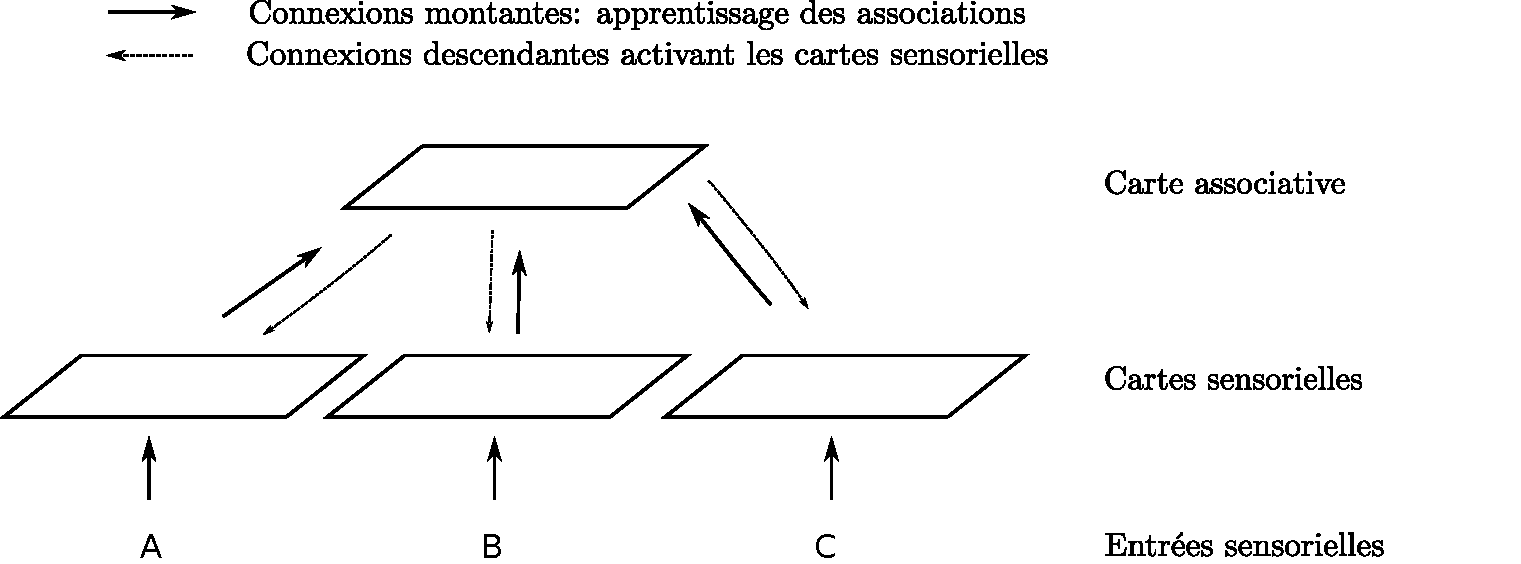
\includegraphics[width=\textwidth]{archi_associative.pdf}
%     \caption{Exemple général d'architecture décentralisée comportant une carte associative. Ces architectures sont utilisées dans des tâches de traitement de données multimodales.
%      Des cartes appelées cartes \emph{sensorielles} ou \emph{modales} prennent des entrées dans plusieurs modalités. Une carte \emph{associative} reçoit des connexions montantes de ces cartes et apprend à associer les activités. Les cartes sensorielles sont connectées à la carte associative par des connexions descendantes pouvant générer une activation dans la carte. Dans la plupart des modèles, les connexions montantes et descendantes n'ont pas le même rôle: les cartes sensorielles ne s'influencent pas entre elles lors de l'apprentissage.
%      Lors de l'utilisation de l'architecture pour de la génération d'entrée sensorielle, alors les connexions descendantes permettent à la carte associative d'activer une carte sensorielle. \label{fig:archi_associative}
%      }
% \end{figure}

\begin{figure}
    \centering
    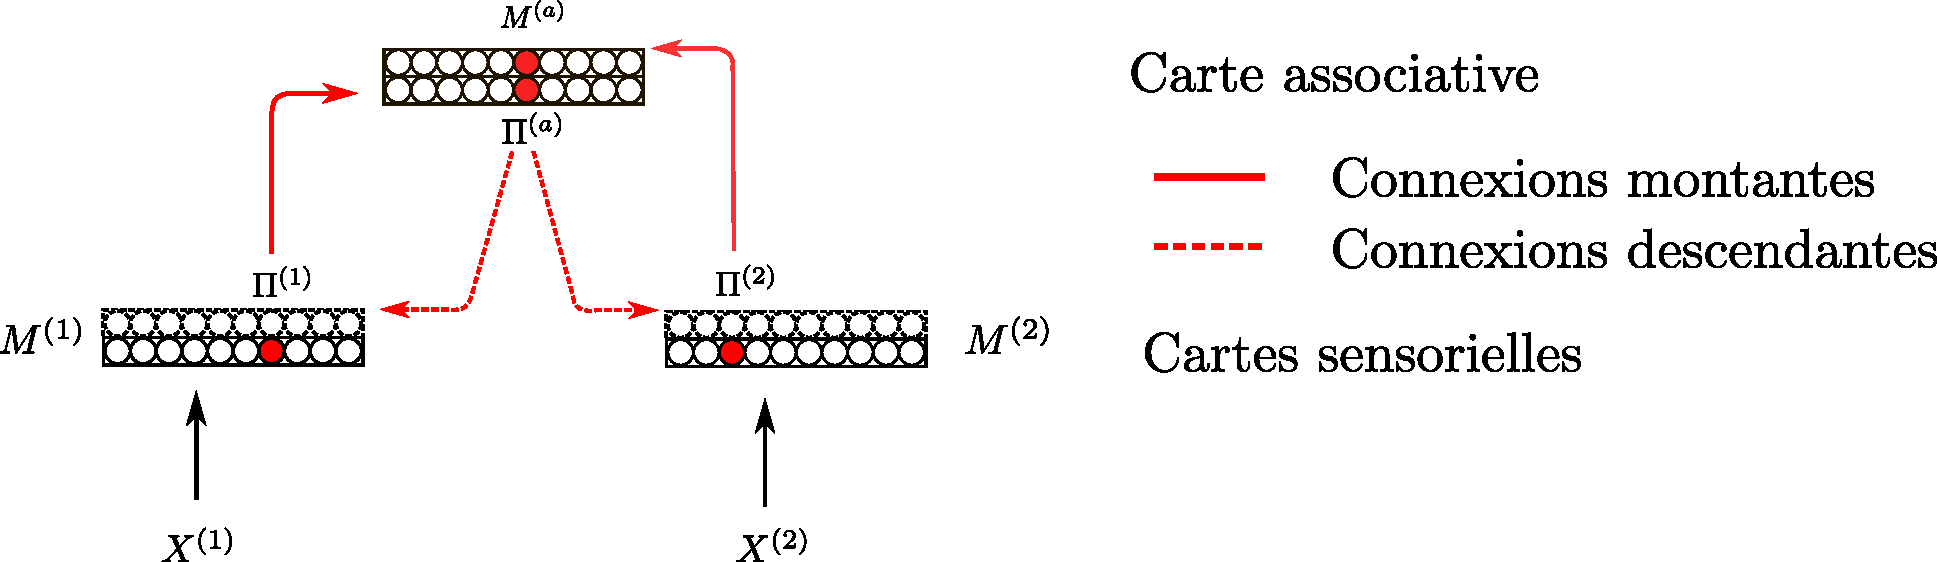
\includegraphics[width=\textwidth]{MCMM.pdf}
    \caption{L'architecture MMCM \cite{dominey13} est une architecture centralisée.
    Les cartes du premier niveau sont les cartes modales, qui reçoivent l'une les mouvements de tête d'un robot, une autre les mouvements de main, la derniere la modalité de parole associée.
    Une carte amodale reçoit les positions des BMUs de chaque carte du premier niveau en tant qu'entrées. 
    \label{fig:mmcm}}
\end{figure}

\begin{figure}
    \centering
    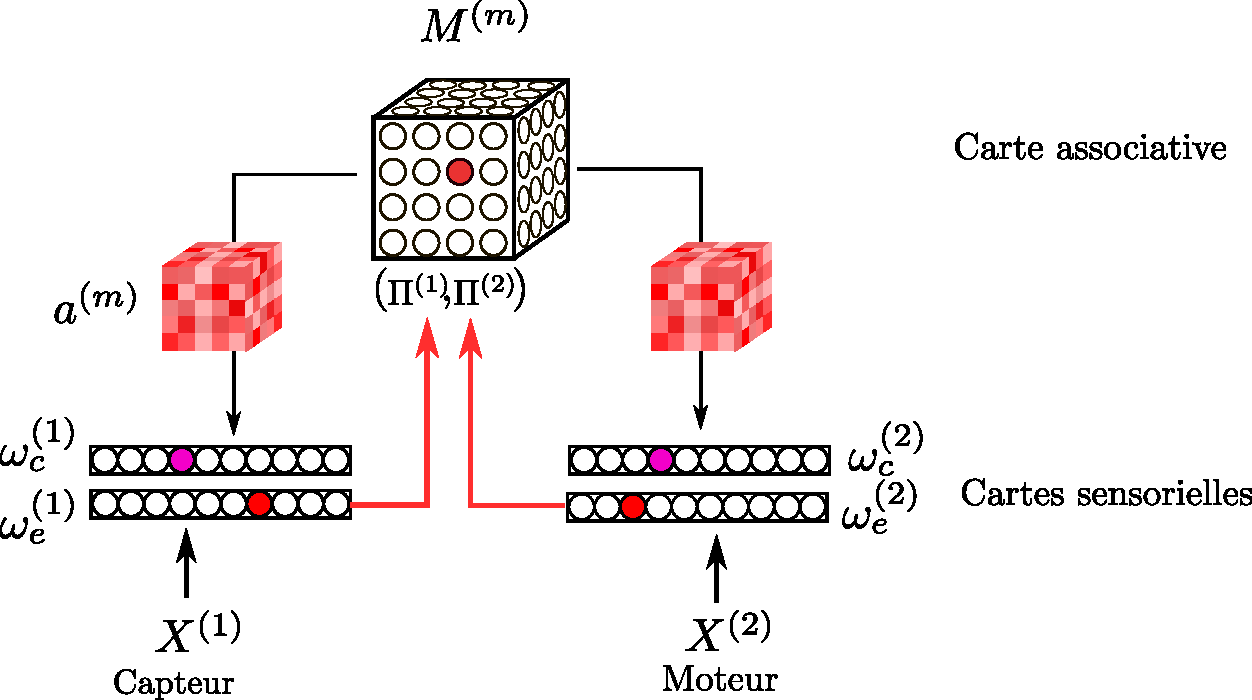
\includegraphics[width=\textwidth]{SOIMA.pdf}
    \caption{L'architecture SOIMA \cite{escobar-juarez_self-organized_2016} est une architecture centralisée.
    \label{fig:SOIMA}}
\end{figure}

Les modèles mentionnés ci-dessus rentrent dans la catégorie non-hiérarchique pour leur possibilité d'activation d'une carte par l'autre. Encore une fois, la position du BMU apparaît chez \cite{dominey13} comme le vecteur de transmission d'information  entre cartes et suffit pour que la coactivation des cartes permettent de réaliser de la mémoire associative. Le modèle SOIMA et le modèle Bijama privilégient la connexion neurone à neurone entre la carte associative et la carte modale, avec une règle d'apprentissage Hebbienne.
Cette mémoire associative est utilisée dans un cadre de données multimodales, avec une notion d'activation d'une carte par l'autre, contrairement aux architectures hiérarchiques citées en section précédentes, utilisées plutot pour des tâches de classification, autrement dit des tâches supervisées.
Dans ces exemples architectures présentées ici, on considère les cartes comme des représentations de leur espace de données qui permettent de la coactivation entres cartes~: une carte de Kohonen prend une fonction générative.

La présence de cartes associatives au sein d'une architecture crée une centralisation de l'information multimodale sur une carte, ce qui nous amène à parler d'apprentissage centralisé. Chaque carte sensorielle ne reçoit aucune information directe d'autres cartes de l'architectures, sauf de la carte associative.

La carte associative tient un role différent dans 
Face aux architectures centralisées, nous pouvons imaginer des architectures décentralisées implémentant des connexions directes entre cartes modales.

\subsubsection{Architectures non-hiérarchiques décentralisées}

Nous avons relevé peu de travaux portant sur des architectures décentralisées, c'est-à-dire comportant des connexions directes entre cartes sensorielles. Un exemple générique d'architecture décentralisée est tracée en figure~\ref{fig:archi_decentralisee}. Les architectures proposées dans tous les travaux que nous avons relevés sont appliquées à de l'apprentissage multimodal.

% \begin{figure}
%     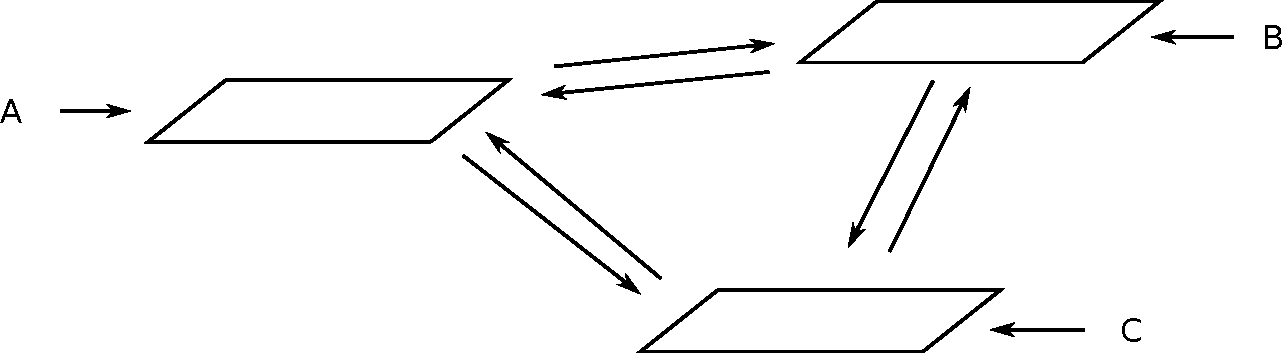
\includegraphics[width=0.9\textwidth]{archi_decentralisee.pdf}
%     \caption{Exemple général d'architecture décentralisée de cartes. Chacune des cartes de l'architecture prend une entrée sensorielle A,B,C. Des connexions entre cartes permettent l'apprentissage d'associations entre modalités. Chacune des cartes peut donc être vue comme une carte multimodale. La façon de gérer les rétroactions entre cartes varie en fonction des travaux et est une problématique majeure dans la construction d'une telle architecture. Ainsi, les cartes apprennent à associer leurs activités seulement après avoir appris les modalités en \cite{khacef_brain-inspired_2020} et conjointement en \cite{johnsson_associative_2009} et \cite{baheux_towards_2014}.\label{fig:archi_decentralisee}}
% \end{figure}

Une telle version d'architecture de cartes non-hiérarchique est développée en \cite{johnsson_associating_2008,johnsson_associative_2009}, sous le nom de A-SOM, \emph{associative self-organizing map}. Encore une fois, le but d'une telle architecture est de faire de l'apprentissage multimodal, en apprenant à associer les activités de cartes sur différentes modalités. La particularité de A-SOM, par rapport à tous les modèles précédemment étudiés, est que l'apprentissage de toutes les cartes et de leurs interactions est réalisé simultanément. Ce modèle décentralisé inclut la possibilité de créer une version d'architecture centralisée à partir des règles d'associations, par exemple \cite{buonamente_hierarchies_2016}. Ainsi, un modèle d'architecture décentralisé est intéressant pour la recherche de nouveaux comportements dans la mesure où il n'impose pas de structure spécifique pour l'architecture. La structure des connexions entre cartes devient alors un paramètre sur lequel on peut complètement agir, contrairement aux architectures centralisées. Le modèle d'architecture est illustré en figure~\ref{fig:asom} pour l'exemple de deux cartes associées. 
Dans ce modèle, chaque ASOM reçoit une entrée $\inpx$ provenant d'une modalité, telle que la texture d'un objet et son image. 
Une carte du modèle A-SOM possède alors deux couches de poids: l'une est relative aux entrées externes $\inpx$ et l'autre relative à l'entrée interne provenant de l'autre ASOM, $X_c$.
Sur ces entrées, les auteurs calculent une activité par couche de poids~: $a_e$ et $a_c$.
L'entrée $X_c$ correspond au vecteur des activations externes $a_e$ des neurones de l'autre carte.
L'interface entre cartes utilisée en A-SOM est donc le champ d'activation des neurones, interface qui avait été utilisée dans l'architecture centralisée SOIMA. Notons que cette interface par transmission d'activation comme entrée d'une carte est équivalente à des connections pondérées par des poids $\w_{cij}$ reliant le neurone $i$ d'une carte au neurone $j$ de l'autre. On a alors $w_c(i) = [\w_{ci1}, \cdots, \w_{ciN}]$.
Lors de l'apprentissage, la mise à jour des poids $\w_e$ et $\w_c$ est réalisée de manière indépendante. 
Le BMU de position $\Pi$ se situe au maximum de l'activité externe et les poids $\w_e$ sont mis à jour comme dans une SOM classique:
$$ \w_e(p) \leftarrow \w_e(p) + \alpha H(\bmu,p)(\w_e(p) - X_e )$$
Les poids $\w_c$ sont mis à jour en fonction de la différence entre activités externes et internes~:
$$ \w_c(p) \leftarrow \w_c(p) + \beta X_c (a_e(p) - a_c(p))$$
Cette règle de mise à jour permet de renforcer le schéma d'activation venant de l'autre carte éappris par un neurone lorsque son activité externe est également forte, et de réduire son impact si le neurone a une activité externe faible. \`A terme, cette règle fait tendre l'activation contextuelle et l'activation externe vers les mêmes schémas.
Pendant l'apprentissage, le calcul d'activité est donc indépendant sur chaque couche de poids, seule la mise à jour insère une dépendance.
Après apprentissage, le but d'une telle structure est de pouvoir couper les entrées externes d'une des cartes et de pouvoir l'activer grâce à la seconde. Le BMU d'une telle carte est alors calculé comme le maximum de l'activité contextuelle. Cette activation permet de générer des prédictions entre modalités.

\begin{figure}
    \centering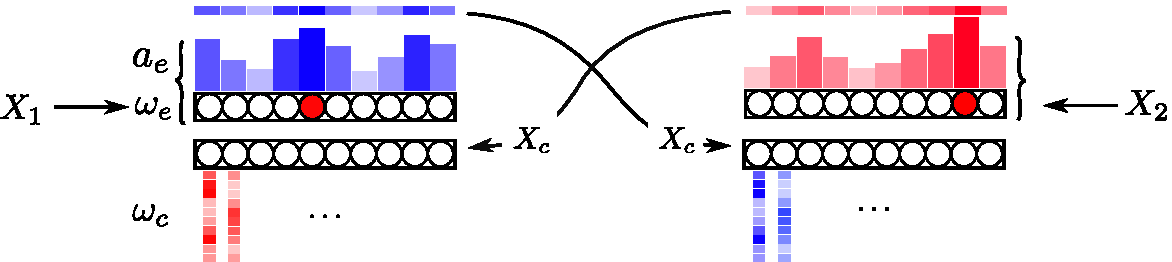
\includegraphics[width=\textwidth]{ASOM.pdf}
    \caption{Le modèle A-SOM \cite{johnsson_associative_2009} associe les activités de différentes cartes. Chaque ASOM prend une entrée modale $X_1$ et $X_2$. Chacune des cartes possède deux couches de poids, une couche $\w_e$ associée aux entrées modales et une couche $\w_c$ associées aux entrées $X_c$ venant de l'autre carte. Lors de l'apprentissage, le calcul des activités sur chaque couche de poids est déconnecté, ce qui permet de gérer les rétroactions. 
    Après apprentissage, une des entrées est coupées. L'activation de cette carte est alors permise par les connexions contextuelles, amenant la carte à prédire une entrée. Les cartes sont représentées en version 1D pour plus de clarté, mais le modèle utilise des cartes 2D.
    \label{fig:asom}}
\end{figure}


\begin{figure}
    \centering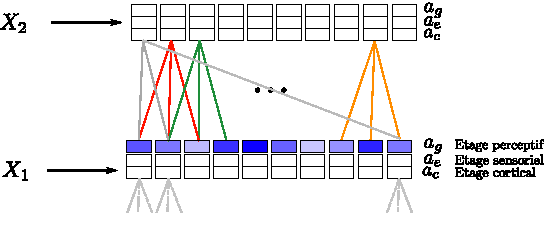
\includegraphics[width=\textwidth]{SOMMA.pdf}
    \caption{Le modèle SOMMA \cite{lefort_unlearning_2011,lefort_apprentissage_2012} associe les activités de différentes cartes, mais en réduisant les champs de réception d'activité aux neurones entourant le neurone situé en position courante. Une seule connexion est représentée, mais toutes les connexions sont réciproques. Contrairement au modèle ASOM, l'activité considérée lors de la transmission est l'activité totale d'une colonne. Les auteurs introduisent un principe de résonance permettant de gérer les rétroactions.
    \label{fig:asom}}
\end{figure}

SOMMA : nous ne nous attarderons pas sur les détails du modèle qui est à base de neurones impulsionnels, éloignés de notre champ d'étude. Néanmoins, le principe de coactivation et de gestion des rétroactions se doit d'être soulevé. Les auteurs utilisent ici comme interface un champ d'activité réduit à une zone de la carte.

Dans \cite{khacef_brain-inspired_2020}. Les auteurs utilisent ici des cartes de Kohonen impulsionnelles, plus directement inspirées de la biologie que les cartes de Kohonen classiques, mais les mêmes principes d'auto-organisation se retrouvent entre les deux modèles. Dans ces travaux, les auteurs apprennent ainsi deux modalités d'un espace multimodal sur deux cartes auto-organisatrices, l'image et le son, puis dans un second temps apprennent les connexions entre neurones en mettant leurs poids à jour à partir des paires d'entrées image-son. Les neurones de chaque carte s'activant sur une même paire d'entrées voient le poids de leur connexion se renforcer, et inversement.
Les auteurs montrent que cette architecture permet d'apprendre les associations d'entrées et peut générer une entrée à partir de l'autre. 
Ce modèle est très simple mais sa mise à jour doit être réalisée en plusieurs étapes~: d'abord les poids des cartes, puis les poids des connexions. 
Cet apprentissage en deux temps était également présent dans l'architecture centralisée de \cite{dominey13}.

L'architecture développée en \cite{lefort_active_2015} implémente également une architecture décentralisée pour de l'apprentissage multimodal. De façon similaire à A-SOM, les auteurs associent plusieurs poids aux neurones d'une carte, chacun des poids étant relatif à un type d'entrée~: l'entrée modale et l'entrée venant d'autres cartes. L'information transmise dans ce cas est une partie de l'activité des neurones, celle située dans un carré centré à la même position que le neurone courant. L'information transmise entre cartes est ainsi également un champ d'activation.

\subsubsection{La mémoire associative comme application des architectures non-hiérarchiques}

Les architectures non-hiérarchiques proposées dans la littérature ont en commun leur application à la mémoire associative de données multimodales.
La fusion de données multimodales, comme définie en \cite{lahat2015} est un enjeu actuel des algorithmes d'apprentissage en robotique. 
Il s'agit d'intégrer les données issues de multiples capteurs au sein d'un même algorithme d'apprentissage.
Il est rare que l'information issue d'un seul capteur apporte toute l'information nécessaire à l'apprentissage et la prise de décision dans un environnement réel. Humainement, notre comportement est en effet influencé par toutes les sources d'informations dont nous disposons.
Dans la mesure ou la recherche en robotique cherche à complexifier les comportements possibles pour les agents, la prise en compte de données de différentes sources est nécessaire. Ces données proviennent d'espace de différentes dimensions comme des images, des capteurs audio, des capteurs tactiles, du texte, des actions. Leur temporalité peut varier~: on veut pouvoir associer des données séquentielles, c'est-à-dire extraire de l'information d'une succession d'entrées, à des données instantanées dans lesquelles seule la valeur de l'entrée compte. La fréquence d'arrivée des données séquentielles varient.
L'enjeu de la fusion de données est de concilier tous ces aspects au sein d'un même algorithme d'apprentissage.

La mémoire associative se définit dans le cadre de la fusion de données multimodale par l'action de prise de décision sur une modalité relativement aux autres.
Les autres modalités peuvent venir améliorer la prise de décision par rapport à la modalité seule. C'est par exemple le cas dans l'effet McGurk \cite{McGurk1976HearingLA}. Alors que la perception de la parole pourrait être uniquement auditive, les psychologues montrent que la présentation du son "ba" à un sujet associée à la présentation d'une video d'une bouche prononçant "ga" amènent le sujet à indiquer qu'il a entendu le son "da". Il est également montré que le fait de lire sur les lèvres en écoutant une personne améliore la compréhension du discours, par exemple dans un environnement bruyant. Il s'agit ici de mémoire associative entre modalités visuelles et auditives.
Cette mémoire associative peut aussi s'utiliser pour prédire d'une modalité par rapport aux autres: les modalités visuelles et auditives vont générer une prise de décision au niveau de la modalité moteur d'un robot et ainsi générer une action par association.
Cette mémoire associative de données multimodales est un des enjeux principaux en robotique fait partie des enjeux fondamentaux pour le développement d'une intelligence incarnée, associée à la notion de développement incrémental.

Les architectures de cartes non-hiérarchiques que nous avons relevées se positionnent dans un cadre de mémoire associative, que ce soit par une motivation bio-inspirée ou par leur but d'implémentation en robotique.
Leur architecture modulaire apparaît comme un moyen de réaliser de la fusion de données à l'échelle de l'algorithme, par opposition à la fusion de données à l'échelle des entrées. Une modalité est alors traitée par un ensemble de cartes~; les autres cartes de l'architectures n'ont accès qu'à une information filtrée et compréhensible par leurs règles d'évolution internes. 
Les cartes hiérarchiques apparaissaient déja comme un moyen de réaliser de la classification sur des données multimodales, par exemple en \cite{mici_self-organizing_2018} et \cite{nawaratne_hierarchical_2020-1}. 
Une carte traite des données spatiales d'un coté, une autre des données temporelles; l'architecture associe la sortie de ces cartes dans la couche finale pour classifier les motifs spatio-temporels. Les cartes du premiers niveaux étaient alors consacrées à la représentation d'une modalité, tandis que la dernière carte est une carte associative apprenant des motifs spatio-temporels liant les deux cartes modales.
Les cartes non-hiérarchiques vont plus loin dans l'application de la mémoire associative car la présence de rétroactions permet de générer une activité au sein d'une carte
modale par ses connexions aux autres cartes, même lorsque l'entrée est manquante. Une carte auto-organisatrice acquiert ainsi une capacité de prise de décision, par son activation.
Cette activation étant lié à des poids représentant la modalité, il est alors possible de prédire une valeur pour la modalité manquante. 
Cette prédiction de modalité est utilisée dans les différents travaux présentés auparavant comme l'application principale de ce type d'architecture et les expériences de validation sont menées autour de la capacité d'une carte modale à prédire de façon précise la modalité à partir des connexions associatives.

- principe louable et intéressant
- souvent restreint à des archis de faible nombre de cartes, alors que si on part sur une motivation bio-inspiré il s'agirait d'implémenter un grand nombre de cartes pour pouvoir le faire


\subsection{Connexions temporelles et architectures de cartes auto-organisatrices}

La capacité de traitement de séquences est un des enjeux de l'application des d'architectures de cartes. Nous avons également relevé des architectures cherchant à unir données spatiales et temporelles en un seul algorithme d'apprentissage. L'objectif d'un algorithme implémentant l'apprentissage de séquence est alors soit de prédire l'élement suivant d'une séquence de données, soit d'extraire des motifs temporels ou spatio-temporels se répétant dans les séquences de données d'entrée. La figure~\ref{fig:mouvement} illustre par exemple ce qu'on attend de l'apprentissage de séquences d'images d'un sportif~: en s'appuyant sur la succession des images présentées à l'algorithme, le but est d'extraire des catégories de mouvements comme "tirer" ou "marcher",ce qui correspond à de la classification des séquences, ou de pouvoir compléter la vidéo en prédisant l'image suivante dans la séquence.
Ainsi, la création d'architectures pour le traitement de données multimodales se rapproche de la question du traitement de séquence. Rappelons également que l'enjeu de la multimodalité se situe en robotique, application dans laquelle les données sont généralement séquentielles.


Cette similarité entre données multimodales et séquentielles n'est pas seulement présente au niveau des objectifs d'applications des architectures de cartes auto-organisatrices mais bien dans la structure même du traitement des données. 
Une solution pour faire de l'apprentissage de séquence peut être de fournir en entrée d'un réseau non plus une donnée instantanée mais une suite de taille fixe de données, sous forme de fenêtre temporelle.
Une autre solution au contraire est de prendre en compte l'état du réseau à l'instant précédent pour effectuer la mise à jour du réseau à l'état courant. Cette solution, implémentée dans de nombreux modèles d'apprentissage, se rapproche de la notion de transmission d'information entre modules d'une architecture, les modules étant ici les états de la carte à deux instants. 
Ces réseaux prenant en compte leur instant précédent pour calculer leur état actuels sont appelés réseaux récurrents ou récursifs. Citons par exemple, en Deep Learning, les RNN (\emph{Recurrent neural networks}), dont les neurones utilisent leur état précédent dans le calcul de leur activité courante.
Plusieurs modèles de cartes auto-organisatrices récurrentes, destiné à l'apprentissage de séquence, ont ainsi été proposés dans la littérature.


L'analyse des cartes récurrentes apparaît ainsi à la fois comme un enjeu de création d'une architecture générale de cartes auto-organisatrices dans la mesure où il s'agit de créer un modèle qui permet d'associer des modules \emph{et} se laisse la possibilité d'y intégrer des connexions récurrentes au même titre qu'une connexion intercartes, et comme une source supplémentaire sur laquelle s'appuyer pour catégoriser les mode de transmission d'information entre cartes. Dans cette section, nous passons en revue différents modèles de cartes récurrentes et nous intéresserons aux modèles multicartes implémentant des connexions récurrentes au même titre que des connexions inter-cartes.

\begin{figure}
    \centering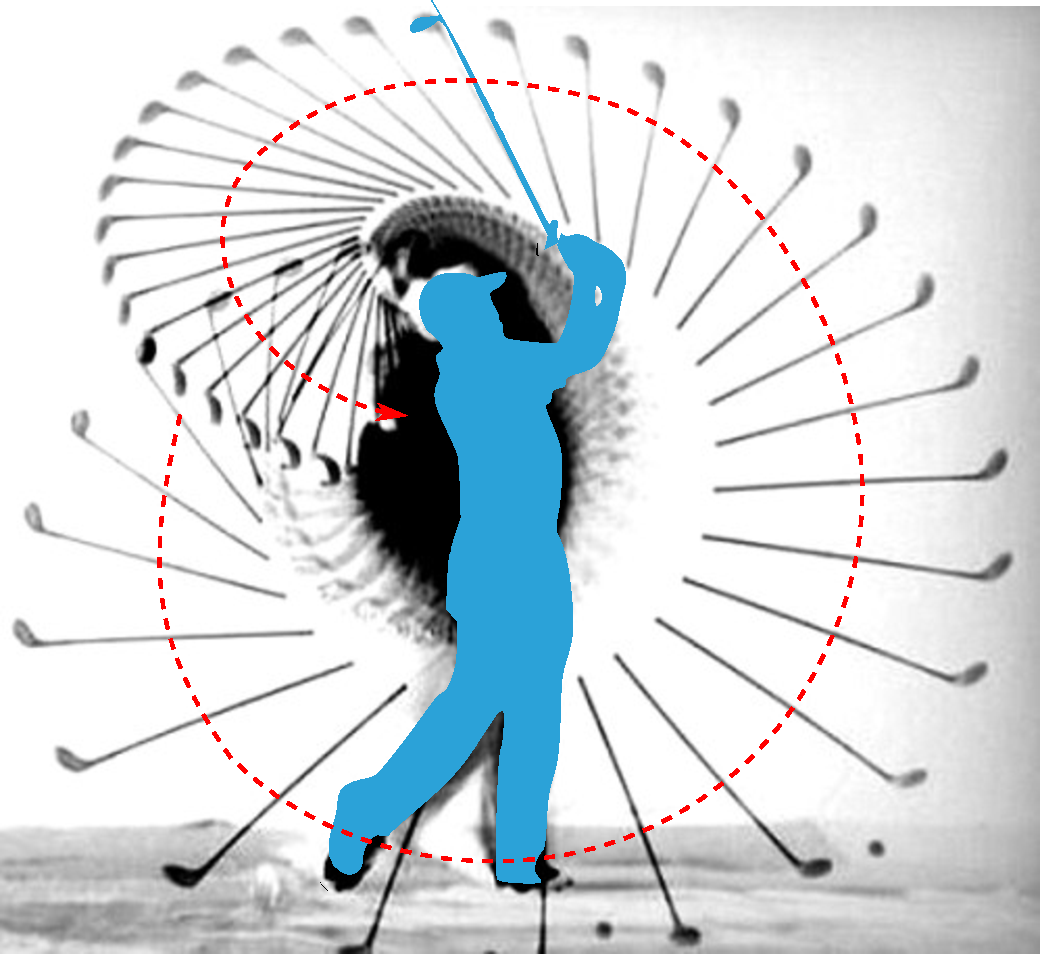
\includegraphics[width=0.6\textwidth]{movment_002.pdf}
    \caption{L'image présentée à un réseau (en bleu) correspond à un instant d'une séquence. L'objectif de l'apprentissage non-supervisé de séquences est d'extraire une représentation d'une séquence d'entrée. Une utilisation commune est la classification de mouvements. La séquence "tirer" sera différente de la séquence "marcher".\label{fig:mouvement}}
 \end{figure}


\subsubsection{Cartes auto-organisatrices récurrentes}



Les modèles de cartes récurrentes existant dans la littérature s'appuient sur la transmission de représentation interne entre itérations. 
L'information transmise entre ces états rejoint les mécanismes relevés dans les architectures multi-cartes: transmission du BMU en tant qu'entrée, transmission d'une activité, transmission du poids du BMU.

Parmi les premiers travaux autour des cartes auto-organisatrices, les cartes de Kohonen Temporelles TKM, dérivées ensuite en \emph{recurrent SOM} \cite{varsta_temporal_2001} utilisent l'activité $a$ d'une carte à l'instant précédent dans le calcul de l'activité à l'instant courant par un modèle d'intégrateur à fuite.
$$a(p,t) = (1-\alpha)a(p,t-1) + \alpha(\inpx_t - \w(p,t)) $$
avec $a$ équivalent ici à une distance modifiée entre un prototype et l'entrée.
Le BMU est alors calculé par $\Pi_t = min(|| a(p,t) || ^2)$.
Le calcul de l'activité revient donc, au lieu de chercher la position donc le prototype $\w(p)$ est le plus proche de l'entrée $\inpx_t$, à chercher une position pour laquelle la distance entre le prototype et l'entrée est faible et pour laquelle la distance calculée par rapport aux entrées précédentes l'était aussi. Il s'agit d'un intégrateur à fuite dans la mesure ou l'influence d'un instant sur les suivants décroit au cours du temps.

D'autres travaux reposent sur la transmission d'une information en tant qu'entrée, prise en compte dans le calcul de l'activité.
Ainsi, les \emph{recursive SOMs} de \cite{Voegtlin2002RecursiveSM} prennent deux entrées~: l'élément de la séquence ainsi qu'un vecteur contenant l'ensemble des activations des neurones de la carte à l'état précédent.
Les travaux de \cite{Buonamente2013SimulatingAW} proposent une version récurrente du modèle A-SOM présenté en section précédente. Le contexte considéré est alors également un ensemble d'activités de neurones. 
MSOM, proposée en \cite{Strickert2005MergeSF} s'appuie sur le poids du BMU. 
A chaque instant, l'entrée de contexte à transmettre à l'état suivant est définie comme une combinaison linéaire entre le poids du BMU courant et le contexte courant.
Enfin, le modèle SOMSD, initialement proposé pour le traitement de données structurées \cite{hagenbuchner_self-organizing_2003} puis étendu au traitement de séquences en \cite{hammer_recursive_2004,hammer_self-organizing_2005} réduit ce contexte à la position de la Best Matching Unit.


Les mécanismes de transmission de contexte entre instants dans les cartes récurrentes s'appuient donc sur les mêmes mécanismes que ceux proposé dans le cadre d'architectures de cartes~: sélection de région de la carte, transmission d'activation, et enfin transmission du BMU.
% Les travaux menés en \cite{fix20} sur le modèle SOMSD montrent qu'une carte récurrente parvient à différencier ses BMUs en fonction de la position de l'entrée dans une séquence et non seulement de la valeur de l'entrée.

\subsubsection{Architectures incluant des connexions temporelles}

Certains modèles s'appuient sur plusieurs cartes de Kohonen connectées, en y ajoutant une notion de traitement de séquences.
en \cite{parisiLL}, les auteurs développent une architecture de deux réseaux auto-organisés appelés \emph{grow when required networks} (GWR). Ces réseaux sont des versions incrémentales de cartes de Kohonen dans lesquelles des neurones sont ajoutés au cours de l'apprentissage, le processus de recherche de BMU restant ensuite similaire à une SOM classique.
Cette architecture utilise deux réseaux GWR pour apprendre des séquences, formant une mémoire épisodique et une mémoire sémantique.
La carte associée à la mémoire épisodique (G-EM) est une version récurrente du GWR, dans laquelle des connexions temporelles entre neurones sont mises à jour en supplément des poids associés aux neurones. Le BMU est alors choisi en fonction de l'entrée courante ainsi que des BMUs précédent. 
La deuxième carte est une version classique du GWR. Elle prend en entrée une séquence de BMUs de la carte G-EM, ainsi que la classe de la séquence courante, afin de mettre à jour ses poids. 
Cette architecture associe ainsi des connexions temporelles récurrentes sur une carte ainsi que des connexions entre cartes.
Cette architecture permet des tâches de \emph{lifelong learning}. 
Le concept d'apprentissage sur le long terme s'intéresse à des systèmes étant mis à jour en ligne, dès qu'ils recoivent une entrée, et dont l'apprentissage n'a pas de limite temporelle fixé. On doit donc avoir un système qui trouve de lui-même une stabilité dans l'apprentissage et qui est capable de s'adapter à de nouvelles entrées.
Dans la plupart des applications en robotique, les entrées présentées à une structure d'apprentissage sont par ailleurs des entrées ayant une relation temporelle. Deux images recues successivement par un capteur visuel seront proches dans l'espace des images. Pour une SOM par exemple, cela pose problème. Les archcitectures de lifelong learning cherchent donc une solution à ces problèmes pour créer une structure autonome, évoluant dans le temps et permettant de réaliser la tâche pour laquelle elle est conçue tout en continuant à être mise à jour, sans oublier les données vues au début de l'apprentissage.
Les auteurs utilisent leur architecture pour de la reconnaissance d'objets. Cependant, lors de l'apprentissage, les données ne sont pas présentées après un tirage aléatoire dans l'espace, mais sont présentés classe par classe~: tous les objets d'une même classe d'abord, etc. Les auteurs montrent que l'architecture est capable de bien prédire la classe d'un objet lors d'un test sur toutes les classes apprises. \`{A} titre de comparaison, une SOM classique apprendrait la classe du premier objet, puis l'oublierait pour se déplier entièrement sur la deuxième classe, etc. A terme, seule la dernière classe apprise est gardée en mémoire.

La motivation de ces modèles multicartes est intéressante~: il s'agit cette fois de voir les deux cartes comme de l'apprentissage à différentes échelles temporelles. L'architecture mélange connexions récurrentes et connexions inter-cartes, ce qui est pertinent dans le cadre de l'apprentissage de séquence, et dans le but de création de systèmes autonomes de cartes auto-organisatrices évoquées par Kohonen. 
Cependant, si sa motivation nous intéresse, le modèle décrit précédemment utilise une logique de vérification externe aux cartes pour ajouter ou nom des neurones. 

Notre démarche s'inscrit dans un objectif d'allier connexions temporelles et connexions intercartes au sein d'une même architecture, sans forcément avoir à différencier ces connexions.
Les travaux autour du modèle A-SOM mentionné précédemment en ont ainsi dérivé une version récurrente \cite{Buonamente2015DiscriminatingAS}. Cette version récurrente est similaire à la version multicarte. Au lieu de considérer l'activité d'une autre carte pour le calcul de l'activité courante d'une carte, les auteurs utilisent l'activité de la même carte à l'état précédent.
Cette structure est appliquée à la prédiction de mouvement. De la même façon qu'une architecture est capable, à partir d'une modalité, de prédire les valeurs correspondant à l'autre modalité, l'architecture incluant une version récurrente peut prédire la fin d'une séquence à partir de son début. La motivation de développer une version récurrente de A-SOM est alors de pouvoir développer des architectures comportant connexions récurrente et connexions intercartes. Nous n'avons pas encore relevé cependant de travaux les intégrant effectivement dans une architecture multicartes.

Les travaux menés en \cite{baheux_towards_2014} (voir figure~\ref{fig:baheux}) ont également cherché à insérer des connexions temporelles au sein d'une architecture de deux cartes. Chaque carte est composée de deux couches de poids. Une des cartes prend une entrée $\inpx(t)$ correspondant à l'observation courante, relative à une première couche de poids, comme une SOM classique. La deuxième couche de poids est relative à l'information interne descendant de la seconde carte, qui est la position du BMU $\bmu_2$ de la deuxième carte. 
La seconde carte recoit deux entrées de la première~: une entrée est la position du BMU $bmu_1(t-1)$ de l'état précédent et la seconde la position du BMU $\bmu_1(t)$ de l'état courant. 
Une activité $a$, gaussienne, est calculée sur chaque couche de poids relativement à son entrée et ces deux activités sont fusionnées en une activité globale à chaque carte :
$$
\begin{cases}
    a_1(t,p) = a(\bmu_2(t),p) + a(\inpx(t),p)\\
    a_2(t,p) = a(\bmu_1(t),p) + a(\bmu_1(t-1),p)
\end{cases} 
$$
Comme chaque carte reçoit en entrée la position de l'état courant du BMU de l'autre carte, il existe une boucle de rétroaction entre carte. Les auteurs laissent alors "résonner" les activités en déplacement petit à petit les BMUs de chaque carte, jusqu'à obtenir un état stable pour les activités, qui est utilisé pour déterminer le BMU final servant à la mise à jour des poids. 
Ce modèle permet alors d'apprendre des séquences d'entrée. Alors qu'une carte simple différencierait les BMUs en fonction de la valeur de l'entrée, ce modèle génère une différenciation des BMUs en fonction de la position d'un élément dans la séquence en plus de sa valeur. 


\begin{figure}
    \centering
    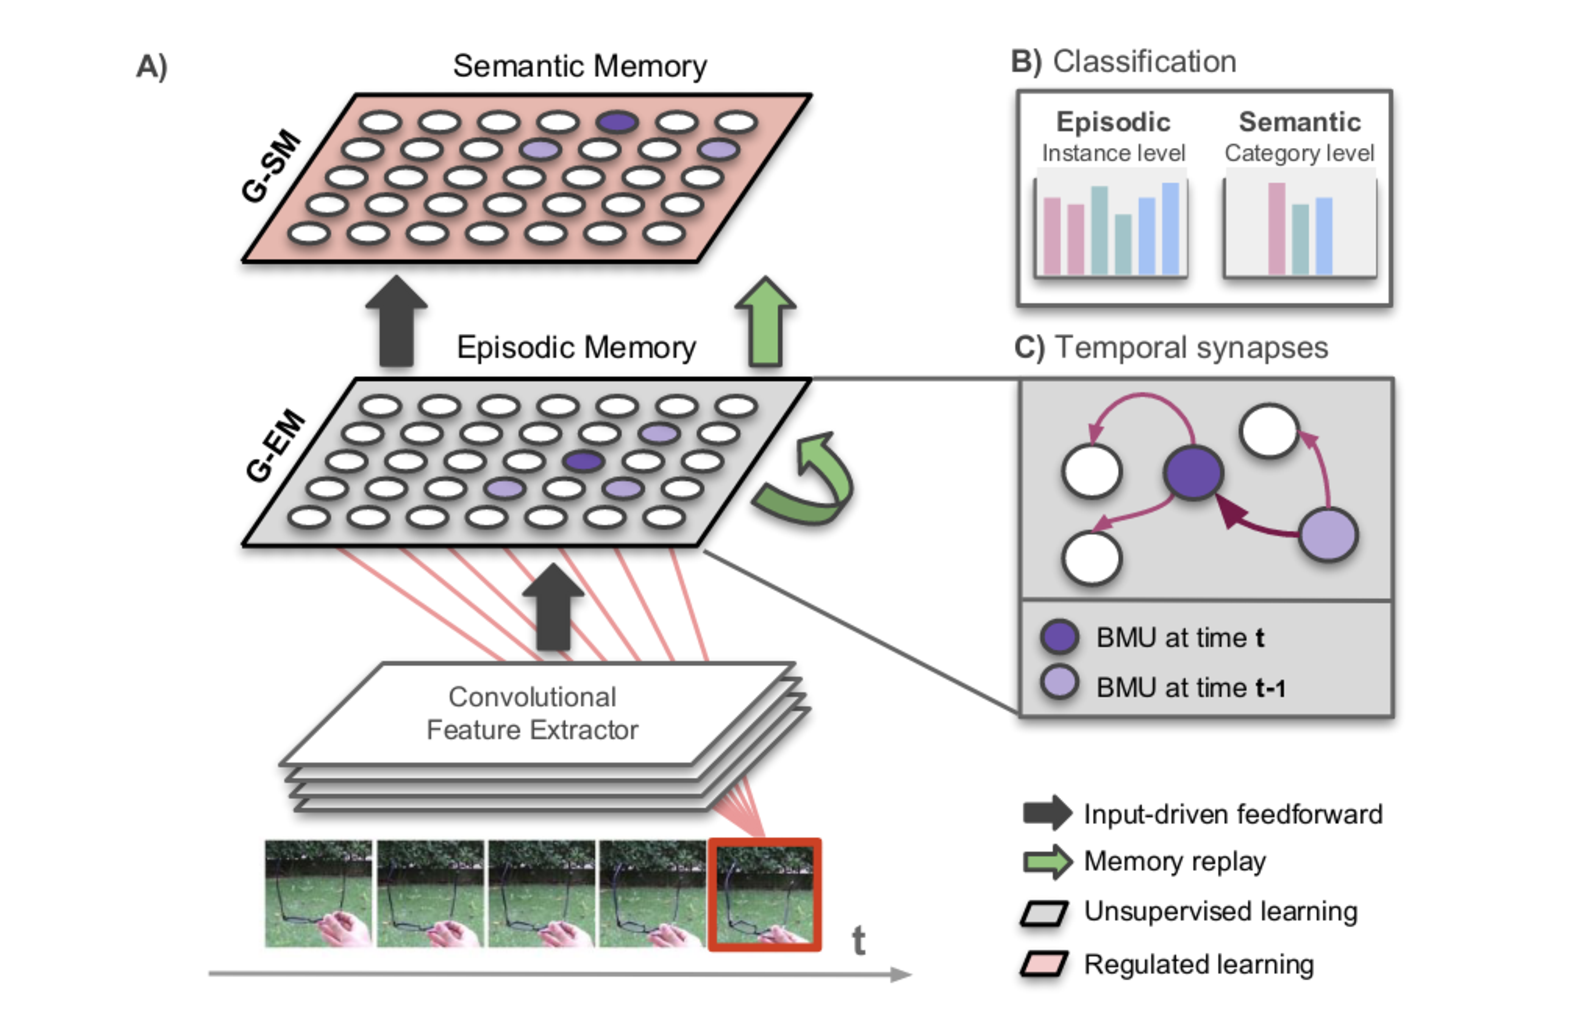
\includegraphics[width=0.8\textwidth]{Parisi_2020.pdf}
    \caption{Architecture \emph{à double mémoire} proposée en \cite{parisiLL}. La couche de mémoire épisodique est un réseau \emph{grow when required (GWR)}, un réseau auto-organisé similaire à une carte de Kohonen, à la différence que les neurones sont ajoutés au fur et à mesure de l'apprentissage. La couche de mémoire sémantique est également un réseau GWR, entraîné à partir des BMUs de la couche épisodique et de la classe de la séquence jouée. L'architecture apprend à reconnaitre plusieurs séquences.\label{fig:gdm_parisi}}
\end{figure}

\begin{figure}
    \centering
    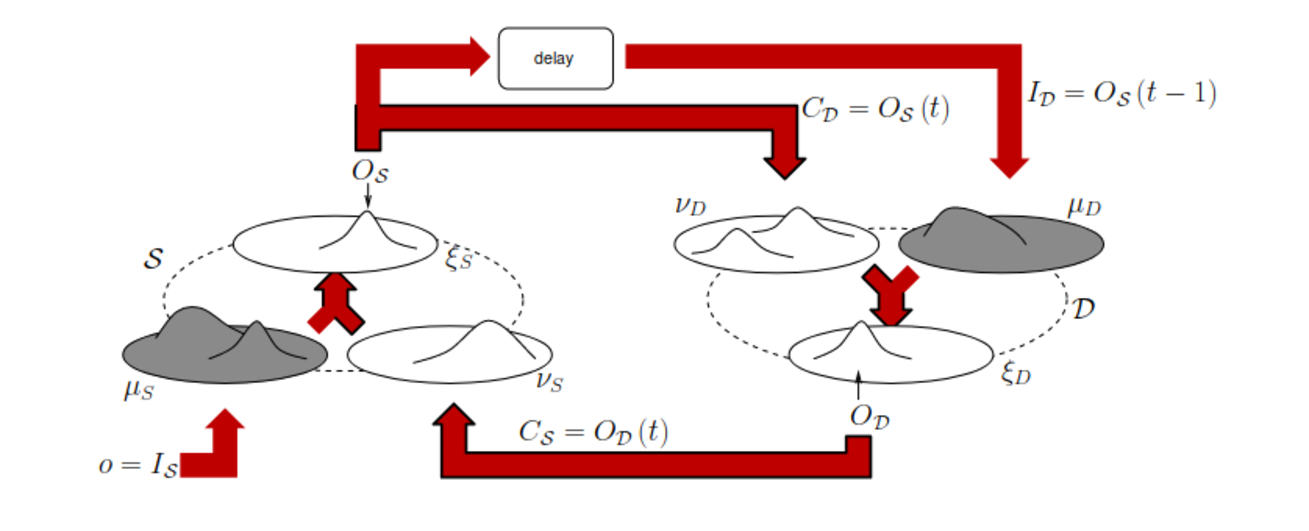
\includegraphics[width=0.8\textwidth]{baheux.pdf}
    \caption{Structures de deux cartes auto-organisatrices communicantes, \cite{baheux_towards_2014}. Chaque carte est composée de trois couches d'activités, représentées séparément sur le schéma: sur la première carte, une activité est relative à l'entrée $o$, l'observation. L'autre activité reçoit une entrée descendant de la seconde carte. Ces deux activités sont fusionnées en une activité globale servant à déterminer un BMU. La seconde carte reçoit ensuite deux entrées venant de la première carte : le BMU de l'état courant et le BMU de l'état précédent. Un système de résonance est mis en place pour gérer les boucles de rétroactions entre BMUs, comme chaque carte reçoit le BMU de l'état courant de l'autre carte en entrée. Ce principe laisse évoluer dynamiquement les activités vers un état stable, utilisé ensuite pour la détermination du BMU final.\label{fig:baheux}}
\end{figure}



\section{Axe de recherche}

Nous avons détaillé la littérature existante en terme d'architecture de SOMs et plus généralement de réseaux de neurones auto-organisés. Nous avons divisé ces architectures en deux grandes catégories~: un format hiérarchique et \emph{feedforward}, et un format non-hiérarchique incluant des rétroactions.
Le format feed forward implique généralement un apprentissage couche par couche. Ce format est très appliqué et permet d'améliorer les capacités de clustering d'une SOM classique, principalement dans le cas ou les données traitées présentent elles-mêmes une structure hiérarchique, telles que des images ou des phrases.
Nous cherchons à développer une architecture plus générale de cartes auto-organisatrices et ne nous placons ainsi pas dans le contexte des Deep SOM mentionné ci-dessus. 
Cependant, nous notons que la position du BMU comme interface entre couche de cartes permet des capacités de calcul.
Nombre de ces architectures sont développées directement dans un but applicatif. On peut ainsi faire la distinction entre un modèle d'architecture, tel que HSOM, qui est générique et applicable à tout type de données, et une structure appliquée, développées spécifiquement pour un type de données.

Opposées à ces architectures hiérarchiques, des architectures reposent sur de l'interaction entre cartes, avec des boucles de rétroaction.
Ces architectures sont moins présentes dans la littérature que les Deep SOM, et cherchent en général à se rapprocher d'un contexte biologique.
Nous nous plaçons plutôt dans la lignée des cartes non-hiérarchiques, sans vouloir cependant copier un aspect biologique.
De façon intéressante, nous remarquons que plusieurs structures non-hiérarchiques sont associées à l'apprentissage de données temporelles. Ces architectures se rapprochent des modèles appelés cartes auto-organisatrices récurrentes, dans lesquels des éléments de calcul d'une carte à une itération données sont réutilisés pour le calcul des itérations suivantes.
Ces architectures non-hiérarchiques dynamiques se divisent en architectures centralisées et décentralisées. La décentralisation des calculs va dans un sens de l'informatique non conventionnelle.

Ces modèles soulèvent également une problématique dans les algorithmes d'apprentissage d'architecture non-hiérarchiques comportant des rétroactions. Dans le cas des neurones impulsionnels, les impulsions des neurones arrivent en différé, une connexion réciproque entre neurones ne pose pas de problème~: les neurones sont traités dans l'ordre des impulsions. Dans le cas de cartes de Kohonen, qui ne repose pas sur des séries d'impulsions, l'information arrive simultanément dans les différentes cartes. L'activité de la carte A influence l'activité de la carte B, mais l'activité de la carte B influence également celle de la carte A, formant une boucle de rétroaction potentiellement infinie. Les architectures mentionnées font le choix d'apprendre d'abord les cartes sensorielles de façon indépendante, puis d'apprendre seulement leurs connexions dans un second temps, décomposant ainsi la boucle. 
La rétroaction est ensuite utilisée en phase applicative pour générer une modalité~: seule une des cartes sensorielle prend une entrée, l'autre carte est considérée comme la sortie de l'architecture et réagit à l'activité des autres cartes. Les rétro-actions ne sont alors pas non plus un problème en phase d'application.

Notons enfin que limites entre les catégories d'architectures que nous avons différenciées dans ce chapitre sont floues. Une architecture décentralisée peut contenir des sous-structures hiérarchiques ou au contraire, une structure hiérarchique de modules décentralisés peut être imaginée.

Parmi ces axes de développement d'architectures, nous choisissons de nous intéresser dans cette thèse à des architectures non-hiérarchiques de cartes.
Les architectures hiérarchiques nous paraissent de bonnes candidates à améliorer les performances d'une SOM sur une application spécifique comme du traitement d'images, tandis que les architectures non-hiérarchiques offrent de nouvelles possibilités de calcul, non envisageables par des SOM classiques, telles que la génération d'entrée, et c'est cet axe que nous souhaitons explorer.
%L'observation d'émergence de calcul dans des systèmes complexes d'apprentissage, introduite au chapitre~\ref{chap:modularite} vient appuyer ce concept.
Peu de travaux ont par ailleurs exploré l'idée d'associer des SOMs en architectures comportant des rétroactions.
Les choix pour la construction d'une telle architecture se situent au niveau de l'interface entre cartes. De nombreux travaux autour des cartes de Kohonen utilisent la position du BMU comme vecteur de l'information transmise entre plusieurs cartes. 
Nous faisons ce choix également. Il apparaît comme une valeur peu coûteuse à communiquer entre cartes, mais qui contient beaucoup d'information sur l'état d'une carte. Cette valeur se présente également comme un cadre homogène de communication intercarte: quelles que soient les entrées sur lesquelles apprend une carte, il sera toujours possible de la connecter à d'autres cartes de l'architecture. 
Enfin, on retrouve l'utilisation de la position du BMU à la fois dans des architectures multicartes et dans les cartes récurrentes comme SOMSD. Le cadre choisi permettrait donc d'intégrer à la fois des cartes classiques et des cartes récurrentes au sein d'une même architecture, offrant encore plus de possibilités de calcul.
Ce modèle de connexions par transmission de position de BMU n'a pas été exploré pour créer des architectures non-hiérarchiques décentralisées. Cette thèse se veut l'exploration de ce modèle.
Nos travaux font ainsi suite à \cite{baheux_towards_2014} sur des architectures récurrentes multimodales utilisant la transmission de la postion du BMU entre des cartes de Kohonen, exploitant la position du BMU comme les travaux sur les cartes récurrentes SOMSD \cite{hagenbuchner_self-organizing_2003,Strickert2003UnsupervisedRS,fix20}.
Les travaux commencés en \cite{baheux_towards_2014}, bien qu'ils exploitent des connexions intercartes, sont similaires à ce qu'on obtiendrait avec une carte récurrente simple, telle que celle décrite en \cite{fix20}.
Nous voulons continuer sur le même modèle, utilisant la transmission du BMU, qui nous apparaît comme une solution compacte et facilement extensible à grande échelle pour construire des grandes architectures, mais en explorant cette fois l'aspect des connexions intercartes.
Par leur motivation, qui est le développement d'un système multi-som, nos travaux se rapprochent aussi des travaux conduits sur l'architecture A-SOM \cite{johnsson_associating_2008, johnsson_associative_2009,gil_sarasom_2015, Buonamente2015DiscriminatingAS}~; notre modèle de carte et d'interface est par contre différent.



\begin{figure*}[b]
    \centering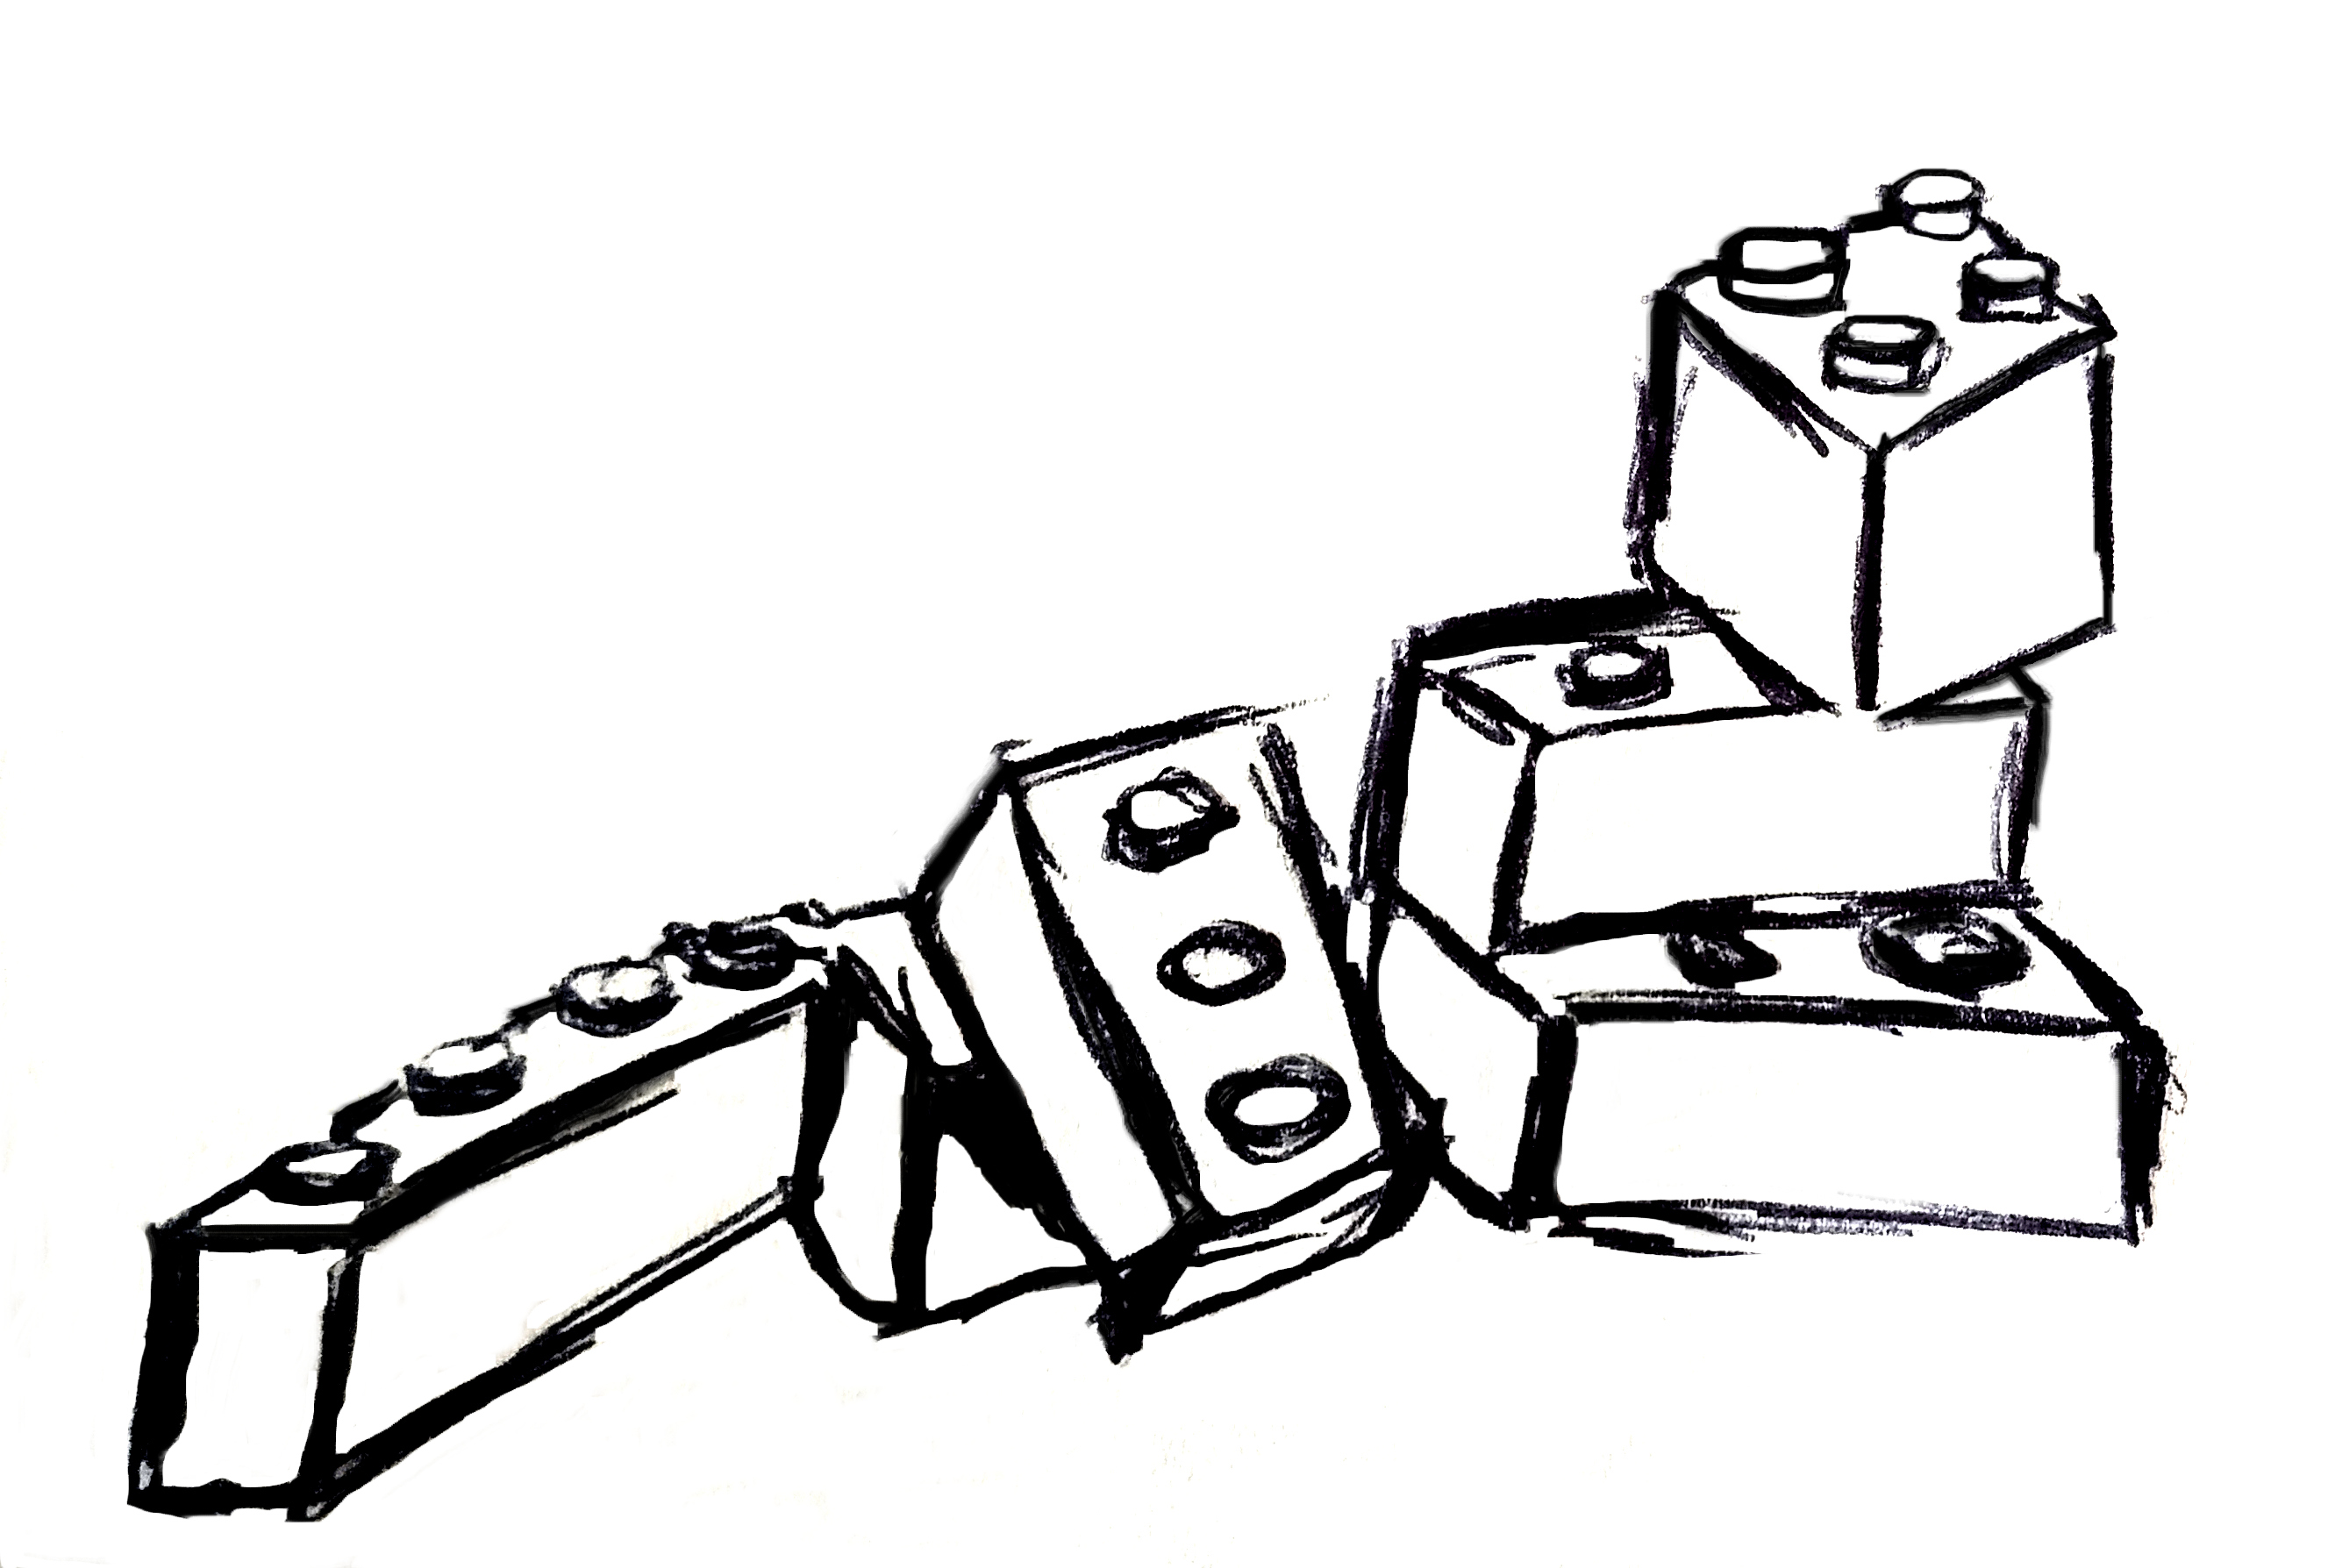
\includegraphics[width=0.6\textwidth]{lego2.jpg}
\end{figure*}

\ifSubfilesClassLoaded{
    \printbibliography
    %\externaldocument{../main.tex}   
}{}
\end{document}